
\newcommand{\rhoabs}{\hyperref[eq:rhoabs-control]{$\rho_{abs}$ 控制条件}}
\newcommand{\supremumf}{\hyperref[eq:supremum-f0-control]{$\sup f_{0}$ 控制条件}}
\newcommand{\lipxOfrho}{\hyperref[eq:lipx_rho_control]{$\operatorname{lip}_x(\rho)$ 控制条件}}
\newcommand{\lipOffVsphere}{\hyperref[eq:lip_Of_f0_in_vsphere_control]{$v$ 球内 $\operatorname{lip}(f_0)$ 控制条件}}
% \newcommand{\rhoabs}{\hyperref[eq:rhoabs-control]{($\rho_{abs}$ control condition)~}}
% \newcommand{\supremumf}{\hyperref[eq:supremum-f0-control]{($\sup f_{0}$ control condition)~}}
% \newcommand{\lipxOfrho}{\hyperref[eq:lipx_rho_control]{($\operatorname{lip}_x(\rho)$ control condition)~}}
% \newcommand{\lipOffVsphere}{\hyperref[eq:lip_Of_f0_in_vsphere_control]{($\operatorname{lip}(f_0)$ in $v$ sphere control condition)~}}
\newcommand{\boundcondition}{\hyperref[de:boundness]{有界条件}}



\chapter{Vlasov-Poisson 系统的局部解}
% \chapter{Local Solutions of Vlasov-Poisson System}

这一章中我们阐述 \cite*{HorstClasssicalI} 采用的通过构造一族误差可以任意小的逼近解来证明 Vlasov-Poisson 系统的局部适定性。具体来说这一章我们将证明以下结论。

% Here we present the standard approximation methods adopted by Horst to investigate the well-posedness of the generalized \eqvp system problem in $N$ dimenstion space. %TODO \cite*{}


\begin{theorem}\textit{($\text{VP}$ 问题的适定性)}
    \label{thm:local-wellposedness}
    假设 $f_{0} \in \mathrm{L}_{1}\left(\bbR^{2 N}\right)$ 满足 \supremumf 和 \lipOffVsphere。那么存在最大的 $0<T^*\leqslant\infty$ 使得 $\text{VP}$ 的解 $ f^{0}$ 在 $[0,T)$ 上存在且唯一。
    
    具体证明见本章最后一节。
    % 且 $f^{0}=\lim_{\varepsilon\rightarrow 0} f^{\varepsilon},$ 在 $I_{1} \times \bbR^{2 N}$ 上一致收敛,其中 $I_{1}$ 是 $I$ 任意的紧子集。


    % Assume that $f_{0} \in \mathrm{L}_{1}\left(\bbR^{2 N}\right)$ satisfies \supremumf and \lipOffVsphere. Assume that $I \subset [0, \infty)$  is an interval with $ 0 \in I $. Then a solution $ f^{0}$ of $\text{VP}^{0}$ exists on $I$, if and only if I satisfies the boundedness condition. In this case $f^{0}$ is unique and $f^{0}=\lim_{\varepsilon\rightarrow 0} f^{\varepsilon},$ uniformly on $I_{1} \times \bbR^{2 N}$ for all compact subsets $I_{1}$ of $I$ $\varepsilon \rightarrow 0$

% 如果 $f_{0}\in C^1(\bbR^{2N})$, 则 $f^{0}\in C^1(I \times \bbR^{2 N})$。

% If $f_{0}$ is continuously differentiable on $\bbR^{2 N}$, then $f^{0}$ is continuously differentiable
% on $I \times \bbR^{2 N}$ and satisfies Vlasov's equation.
% Remark. In view of theorem (2.8) this proves global existence of a solution of $P^{0}$ for $N=1,2$ and at least local existence for $N \geqslant 3$
\end{theorem}


% 该方法适用于 $N\in \bbZ, N \geqslant 1$ 维空间,证明前还需要对我们在介绍中引入的定义进行扩展,即定义 Vlasov-Poisson 系统在 $N$ 维空间中的形式及解在何种意义下成立,并且说明积分核奇异性被削弱之后的解如何定义。对 Vlasov 类型的问题,我们通常说的经典(Classical)解的意义即为对特征线常微分方程,任意给定初值均有唯一解,特征线在 Vlasov 类型问题中的重要性,我们将会在对解的定义中感受到。


因为积分核有奇异性,常用的分析方法无法直接给出适定性的结果,所以 \cite{HorstClasssicalI} 的想法是 (i) 先构造逼近解,也就是解决 $\text{VP}^\varepsilon$ 问题,由于 $\text{VP}^\varepsilon (\varepsilon >0)$ 问题中核函数的奇异性被移除了,经典的分析手段告诉我们逼近解的存在性 $\text{VP}^\varepsilon (\varepsilon >0)$ ; (ii) 逼近解的一些重要估计,例如 $\operatorname{lip}_x (\vE(t))$ 等;(iii) 估计逼近解之间的误差,得出逼近解的一致收敛性。

在此之前我们需要做一些定义上的扩展,第一节先给出了 $\text{VP}^\varepsilon$ 问题给出的逼近解的定义。第二节给出在\supremumf 下,逼近解的一些估计,主要是对 $\|\vE^\varepsilon(t)\|_\infty$, $\|\rho^\varepsilon(t)\|_\infty$ 和 $\sup \{|\vect{V}^\varepsilon(r,0,\vx,\vv)-\vv| \bigg|\vx,\vv \in \bbR^N, 0\leqslant r \leqslant t \}$ 的一致控制。第三节给出对 $\vE^\varepsilon$ Lipschitz 常数的一致控制。第四节说明 $f^\varepsilon$ 确实在 $I\times \bbR^N \times \bbR^N $ 上当取极限 $\varepsilon\rightarrow 0 $ 时一致收敛到 $f^0$,主要依据是特征线确实随着 $\varepsilon\rightarrow 0$ 一致收敛,这是在本章最后的第四节完成的。




% 然后则是第三节,证明这点需要对密度 $\rho^\varepsilon$ 的 $\mathrm{L}^1$ 和 $\mathrm{L}^\infty$ 范数及其的 Lipschitz 连续性。这里我们需要另外的\lipOffVsphere 来补充需要的初值的 Lipschitz 连续性。


\begin{figure}[h]
    \centering
    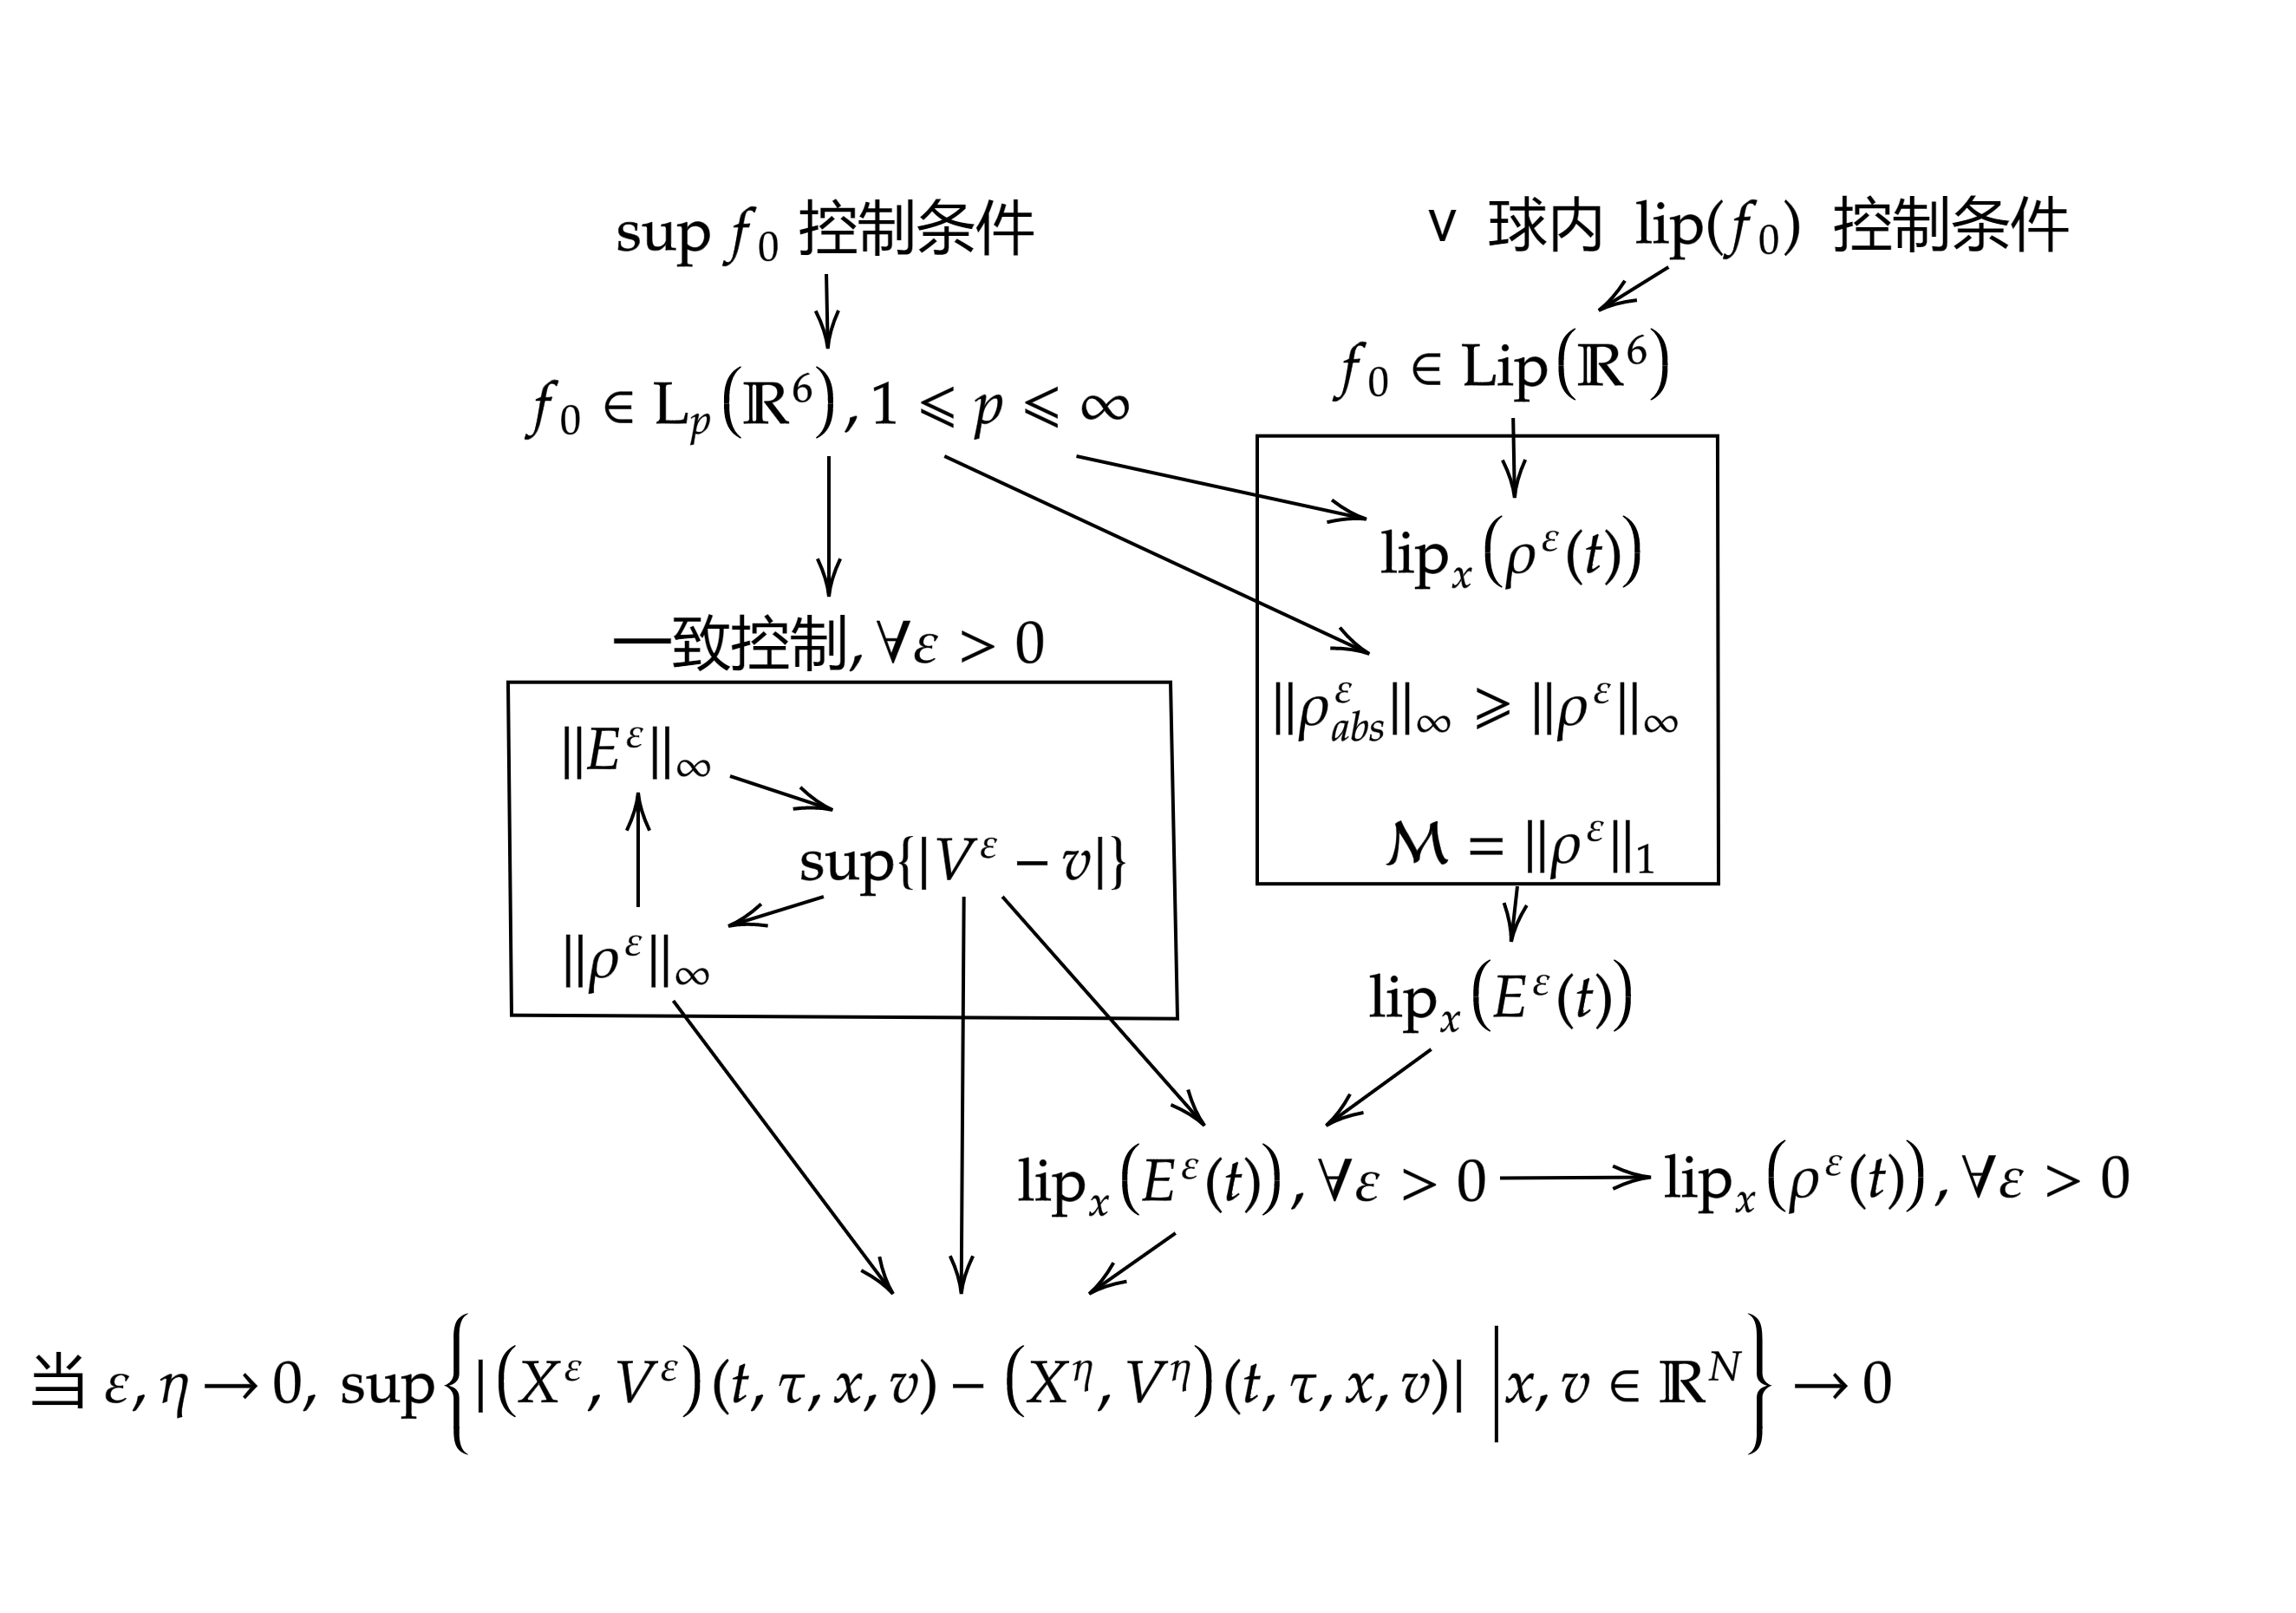
\includegraphics[width=1.0\textwidth]{diagram.png}
    \caption{图中所示为证明适定性过程中各个命题证明的前后序列,其中箭头表示我们证明命题的前后关系,而不是逻辑上的充分关系;出现在图中的变量表示存在 $H\in C_+(I)$ 中函数对其控制,$\forall \varepsilon>0$ 表示对 $\varepsilon$ 一致控制。}
    \label{fig:diagram}
\end{figure}

% 以 $\|\rho^\varepsilon\|_\infty$, $h_v^\varepsilon(t)$ 及 $\operatorname{lip}_x (\vE^\varepsilon(t))$ 三者的一致控制为基础,我们得以证明区间有界条件与局部解存在互为充要条件,从而刻画 Vlasov-Poisson 方程的适定性。

\section{定义扩展}
% \section{Definition Preparation}
\begin{equation}
    \label{eq:vp_ndim}
    \text { (VP \& RVP) }\left\{\begin{array}{l}
    \partial_{t} f+\vect{a}(\vv ) \cdot \nabla_{x} f+\vE \cdot \nabla_{v} f=0 \\
    \vE(t, \vx)=\mu\int \frac{\vx - \vect{y}}{|\vx - \vect{y}|^N} \rho(t,\vx) \mathrm{d} \vx %\quad =-\nabla_{x} \phi(t, \vx)\\
    %\phi= \mu \frac{1}{|\vx|^{N-1}} *\rho
\end{array}\right.\end{equation}


 $f_{0} \in \mathrm{L}_{1}\left(\bbR^{2 N}\right)$ 总是表示所考虑的偏微分问题的初值条件。 用 $m:=\|f_{0}\|_{1}$ 表示初始质量, 即相空间分布函数的 $\mathrm{L}_1$ 范数。
% We always use $f_{0} \in \mathrm{L}_{1}\left(\bbR^{2 N}\right)$ to denote the initial data for the problem to be considered. Let $m:=\|f_{0}\|_{1}$ denote the initial mass, \textit{i.e.} $\mathrm{L}_1$ norm of initial phase function.
场函数积分核的奇性我们用参数 $\varepsilon$ 进行了削弱,新的积分核为
% The singularity of the field integral kernel is modified with a parameter $\varepsilon$ as follows.
$$\vect{e}^{\varepsilon}(\vect{z})=\gamma \cdot \frac{\vect{z}}{\left(|\vect{z}|^{2}+\varepsilon\right)^{N / 2}},~ \quad ~ \vect{z} \in \bbR^{N}, \varepsilon \geqslant 0$$
参数 $\varepsilon$ 弱化了场函数的奇性,相当于重新定义了新的偏微分方程 $\text{VP}^\varepsilon$ 问题,下面拓宽对它的定义。
% Since we have weakened the singularity by the $\varepsilon$, the solutions to the $\text{VP}^\varepsilon$ are redefined as follow.

\begin{definition}\textit{($\text{VP}^\varepsilon$ 问题及其解)}
% \begin{definition}\textit{(The solution of $\text{VP}^\varepsilon$)}
    假设 $I \subset[0, \infty)$ 是一个含 $0$ 的区间。称 $f^{\varepsilon}: I \times \bbR^{2 N} \rightarrow \bbR$ 是 $\text{VP}^{\varepsilon}(\varepsilon \geqslant 0 \text { 固定})$ 在 $I$ 上的解, 如果它满足下面的条件:
%    Assume that $I \subset[0, \infty)\text { is an interval with } 0 \in I .\text { We say that }$ $f^{\varepsilon}: I \times \bbR^{2 N} \rightarrow \bbR$ is a solution of problem $\text{VP}^{\varepsilon}(\varepsilon \geqslant 0 \text { fixed })$ on $I$, if

    \begin{enumerate}[(1)] 
        \item $f(0,\cdots) = f_0$
        \item 对任意的 $t \in I, \vx \in \bbR^{N}$ 有下列映射的可积性, $\left((\vect{y},\vect{u}) \mapsto \vect{e}^{\varepsilon}\left(\vx-\vect{y}\right) \cdot f^{\varepsilon}(t, \vect{y},\vect{u})\right) \in \mathrm{L}_{1}\left(\bbR^{2 N}, \bbR^{N}\right)$ 
        % \item $\left((\vect{y},\vect{u}) \mapsto \vect{e}^{\varepsilon}\left(\vx-\vect{y}\right) \cdot f^{\varepsilon}(t, \vect{y},\vect{u})\right) \in \mathrm{L}_{1}\left(\bbR^{2 N}, \bbR^{N}\right)$ for all $t \in I, \vx \in \bbR^{N}$
        \item $\vE^{\varepsilon}\left(t, \vx\right):=\iint_{\bbR^6}  \vect{e}^{\varepsilon}\left(\vx-\vect{y}\right) \cdot f^{\varepsilon}(t, \vect{y},\vect{u}) \mathrm{d} \vect{y} \mathrm{d}\vect{u}$ 用来替换原来的有奇异性的场函数积分核。要求 $\text{VP}^\varepsilon$ 问题解的分布函数产生的 $\vE^{\varepsilon}$ 在 $I \times \bbR^{N}$ 上连续,且对任意的 $t \in I$ 有 $\vE^{\varepsilon}(t, \cdot) \in \mathrm{C}_{b}^{0}\left(\bbR^{N}, \bbR^{N}\right) \cap \operatorname{Lip}\left(\bbR^{N}, \bbR^{N}\right)$ 并存在
        $C_\rho^{\varepsilon}, C_{lip(E)}^{\varepsilon} \in C_{+}(I)$ 使得对任意的 $t \in I$
        \[
        \left\|\vE^{\varepsilon}(t, \cdot)\right\|_{\infty} \leqslant C_{ E}^{\varepsilon}(t), \quad 
        \operatorname{lip}\left(\vE^{\varepsilon}(t, \cdot)\right) \leqslant C_{\operatorname{lip}(E)}^{\varepsilon}(t)
        \]
        \item 
        解 $f^{\varepsilon}$ 通过 $\text{VP}^\varepsilon$ 特征线的常微分问题来定义,这是因为沿特征线有 $f^\varepsilon$ 不变的特性. 具体而言场修正后的特征线方程如下, 
        % The solution $f^{\varepsilon}$ is defined according to the characteristic trajectories of the $\text{VP}^\varepsilon$ problem, along which the value $f^\varepsilon$ should not change. The characteristic under the modified electrical field $\vE^\varepsilon$ is 
        \begin{equation}
            \dot{\vect{X}}^\varepsilon=\vect{V}^\varepsilon, \dot{\vect{V}}^\varepsilon=\vE^{\varepsilon}\left(t, \vect{X}^\varepsilon\right), \quad t \in I,
        \end{equation}
        
        它对任一初值 $\vx,\vv\in\bbR^N$ 在 $I$ 上均有唯一解,这由 (3) 中的有界条件保证。 $f(t,\vx, \vv)$ 通过沿特征线给定常微分方程的初值状态(实际是末值)来追溯到特征线 $t=0$ 时刻的 $f_0$ 值, $\vect{X}^\varepsilon(t)= \vx, \vect{V}^\varepsilon(t)= \vv$, 即
        % which has a unique solution on $I$ for any initial value thanks to the regularities given in (3). $f(t,\vx, \vv)$ is given by the characteristic with initial condition $\vect{X}^\varepsilon(t)= \vx, \vect{V}^\varepsilon(t)= \vv$, \textit{i.e.}
        \[
        f^{\varepsilon}(t, \vect{X}^\varepsilon(t), \vect{V}^\varepsilon(t))=f^{\varepsilon}(0, \vect{X}^\varepsilon(0), \vect{V}^\varepsilon(0))=f_{0}(\vect{X}^\varepsilon(0), \vect{V}^\varepsilon(0)), \quad t \in I
        \]
        如果 $I=[0, \infty)$, $f^{\varepsilon}$ 被称为一个全局(时域)解,否则被称为局部解。
        % if $I=[0, \infty)$, $f^{\varepsilon}$ is named a global solution, otherwise a local solution.
    \end{enumerate}

\end{definition}


% $C_{b}^{k}\left(\bbR^{M}, \bbR^{L}\right):=\left\{f: \bbR^{M} \rightarrow \bbR^{L} | f \text { is } k$ times continuously differentiable \right.
% and all these derivatives are bounded $\}, \quad 0 \leqslant k \leqslant \infty$




\begin{theorem}\textit{($\text{VP}^\varepsilon$ 当 $\varepsilon>0$ 时的适定性)}
% \begin{theorem}\textit{(Well-posedness of $\text{VP}^\varepsilon$ when $\varepsilon>0$)}
\label{thm:epsilon-greater-0}
如果 $\varepsilon>0$, 那么存在着 $\text{VP}^{\varepsilon}$ 的唯一全局解 $f^\varepsilon$。如果 $I\subset[0, \infty)$ 是一个含 $0$ 的区间,那么 $\left.f^{\varepsilon}\right|_{I \times \bbR^{2N}}$ 是 $I$ 上的解,并且该解唯一。
% If $\varepsilon>0,$ there exists a unique global solution $f^\varepsilon$ of $P^{\varepsilon}$. If $I$ is a subinterval of $[0, \infty)$ with $0 \in I$ then $\left.f^{\varepsilon}\right|_{I \times \bbR^{2N}}$ is a solution on $I$ and this solution is unique.
\end{theorem} 
\begin{proof}
    此处可以引用 \cite*{Horst1975}  硕士论文中采用的方法,但以此得到的 $H_E^\varepsilon(t),H_{lip(E)}^\varepsilon(t)$ 是 $\varepsilon$ 的负幂的乘积,故而注意对 $\varepsilon=0$ 的情况不适用。
    % The result can be acquired with the methods of [11].
\end{proof}

\begin{definition}
    假设 $f^{\varepsilon}$ 是 $\text{VP}^{\varepsilon}(\varepsilon \geqslant 0 \text{固定})$ 在 $I$ 上的解. 对任意的$t_{0} \in I, (\vx,\vv) \in \bbR^{2 N}$, 记 $\vect{X}( s , t_0,\vx,\vv), \vect{V}( s , t_0,\vx,\vv) : I \times I \times \bbR^N \times \bbR^N \rightarrow \bbR^n$ 为特征线常微分方程满足以下初值问题的解。
    $$\vect{X}^{\varepsilon}\left(t_{0}, t_{0}, \vx,\vv \right)=\vx, \quad \vect{V}^{\varepsilon}\left(t_{0}, t_{0}, \vx,\vv \right)=\vv$$

    % 该定义可以直接导出对任意的 $t_{1}, t_{2}, t_{3} \in I$ 有,
    % $$(\vect{X}^{\varepsilon}, \vect{V}^\varepsilon) \left(t_{1}, t_{2}, \cdot\right) \circ  (\vect{X}^{\varepsilon}, \vect{V}^\varepsilon) \left(t_{2}, t_{3}, \cdot\right)  =(\vect{X}^{\varepsilon}, \vect{V}^\varepsilon)\left(t_{1}, t_{3}, \cdot\right)$$
    
    % 特别地当 $t_3 = t_1$ 我们有 $(\vect{X}^{\varepsilon}, \vect{V}^\varepsilon) \left(t_{1}, t_{2}, \cdot\right)$ 的反函数是 $(\vect{X}^{\varepsilon}, \vect{V}^\varepsilon) \left(t_{2}, t_{1}, \cdot\right)$.

    % Assume $f^{\varepsilon}$ is a solution of $\text{VP}^{\varepsilon}(\varepsilon \geqslant 0 \text { fixed) on } I$. For any $t_{0} \in I, (\vx,\vv) \in \bbR^{2 N}$, let $\vect{X}( s , t_0,\vx,\vv), \vect{V}( t , t_0,\vx,\vv) : I \times I \times \bbR^N \times \bbR^N \rightarrow \bbR^n$ denote the solution of the characteristic ordinary differential system that
    % satisfies the initial condition
    % $$\vect{X}^{\varepsilon}\left(t_{0}, t_{0}, \vx,\vv \right)=\vx, \quad \vect{V}^{\varepsilon}\left(t_{0}, t_{0}, \vx,\vv \right)=\vv$$
\end{definition}

\begin{lemma}\textit{(特征线相关性质)}
% \begin{lemma}\textit{(Features of characteristcs)}

特征线有以下性质:
% Then the following statements are valid
\begin{enumerate}[(i)]
    \item $\vect{X}^{\varepsilon},\vect{V}^{\varepsilon}$ 在 $I \times I \times \bbR^{2N}$ 上连续
    % \item $\vect{X}^{\varepsilon},\vect{V}^{\varepsilon}$ are continuous on $I \times I \times \bbR^{2N}$
    \item 给定 $t_{1}, t_{2} \in I$ 函数 $\vect{X}^{\varepsilon}\left(t_{1}, t_{2}, \cdot\right)$ 是 $\bbR^{2N}$ 映到 $\bbR^{2N}$ 上的保测度(Lebesgue)同胚。
    % \item For any $t_{1}, t_{2} \in I$ the function $\vect{X}^{\varepsilon}\left(t_{1}, t_{2}, \cdot\right)$ is a (Lebesgue) measure preserving homeomorphism of $\bbR^{2N}$ onto $\bbR^{2N}$.

    % \item 若 $\frac{\partial}{\partial \vx} E^{\varepsilon}\left(t,\vx\right)$ 存在并在 $I \times \bbR^{N}$ 上连续,则 $\vect{X}^{\varepsilon}$ 对于 $s,t, \vx,\vv$ 均连续可导 %并满足一阶偏微分方程组 
    % $$\frac{\partial}{\partial t_{1}} \vect{X}^{t}\left(t, t_{1}, x\right)+x_{v} \cdot \nabla_{x} \vect{X}^{t}\left(t, t_{1}, x\right)+E^{\varepsilon}\left(t_{1},\vx\right) \cdot \nabla_{v} X_{i}^{t}\left(t, t_{1}, x\right)=0$$

    % \item If $\frac{\partial}{\partial x_{3}} E^{t}\left(t,\vx\right)$ exists and is continuous on $I \times \bbR^{N},$ then $\vect{X}^{\varepsilon}$ is continuously differentiable with respect to all arguments and satisfies the system of first order partial differential equations
    % $$\frac{\partial}{\partial t_{1}} \vect{X}^{t}\left(t, t_{1}, x\right)+x_{v} \cdot \nabla_{x} \vect{X}^{t}\left(t, t_{1}, x\right)+E^{\varepsilon}\left(t_{1},\vx\right) \cdot \nabla_{v} X_{i}^{t}\left(t, t_{1}, x\right)=0$$
    \item 因为沿特征线偏微分方程的待求函数值 $f^{\varepsilon}$ 不变,我们有对任意的 $t, t_{1} \in I, x \in \bbR^{2N}$
    % As $f^{\varepsilon}$ is an integral of $(1.2 .1),$ we have for all $t, t_{1} \in I, x \in \bbR^{2N}$
    
    $$f^{\varepsilon}\left(t, \vect{X}^{\varepsilon}\left(t, t_{1}, \vx, \vv\right), \vect{V}^{\varepsilon}\left(t, t_{1}, \vx, \vv\right)\right)=f_0\left(\vect{X}^{\varepsilon}(0, t_1, \vx, \vv)\right)$$

    \begin{equation}
        \label{eq:characteristic-traceback}
    f^{\varepsilon}(t, \vx, \vv)=f_{0}\left(\vect{X}^{\varepsilon}(0, t, \vx, \vv), \vect{V}^{\varepsilon}(0, t, \vx, \vv)\right)
    \end{equation}

    于是对任意的 $t \in I$, $f^{\varepsilon}(t, \cdot)$ 和 $f_{0}$ 有着相同的值域 , 因此 $f^{\varepsilon} \geqslant 0$ 当且仅当 $f_{0} \geqslant 0$ 并且 $\sup \left|f^{\varepsilon}(t, \cdot,\cdot)\right|=\sup |f_{0}|$。 $f^{\varepsilon}$ 在 $I \times \bbR^{2N}$ 上连续,当且仅当 $f_{0}$ 在 $\bbR^{2N}$ 上连续。% 如果 $\nabla_{x} E^{\varepsilon}\left(t,\vx\right)$ 存在并在 $I \times \bbR^{N},$ 上连续,由 (iii) 和方程 \ref{eq:characteristic-traceback} 得到 $f^{\varepsilon}$ 是可导的(连续可导的)当且仅当 $f_{0}$ 是可导的(连续可导的),并且这种情况下 $f^{\varepsilon}$ 确实满足原偏微分方程。
    % Therefore $f^{\varepsilon}(t, \cdot)$ has the same range as $f_{0}$ for all $t \in I$, hence $f^{\varepsilon} \geqslant 0,$ if and only if $f_{0} \geqslant 0$ and $\sup \left|f^{\varepsilon}(t, x)\right|=\sup |f_{0}(x)| . f^{\varepsilon}$ is continuous on $I \times \bbR^{2N},$ if and only if $f_{0}$ is continuous on $\bbR^{2N}$. If $\nabla_{x} E^{\varepsilon}\left(t,\vx\right)$ exists and is continuous on $I \times \bbR^{N},$ then (iv) and $(1.4 .4)$ imply
    % that $\Phi^{c}$ is differentiable (continuously differentiable), if and only if $f_{0}$ is differentiable (continuously differentiable) and in this case $f^{\varepsilon}$ satisfies the partial differential equation

    % $$ \frac{\partial}{\partial t} f^{\varepsilon}(t, x)+\vv\cdot \nabla_{x} f^{\varepsilon}(t, \vx, \vv)+\vE^{\varepsilon}\left(t, \vx\right) \cdot \nabla_v f^{\varepsilon}(t, \vx, \vv)=0$$

    \item  %(ii) 和方程 \ref{eq:characteristic-traceback} 表明
    对任意的 $t, t_{1} \in I$ 和任何可测函数$\sigma: \bbR^{2N} \rightarrow \bbR^{M}$,我们有 $\sigma \in \mathrm{L}_{1}\left(\bbR^{2N}, \bbR^{M}\right)$ 的充要条件是 $\sigma \circ (\vect{X}^{\varepsilon},\vect{V}^{\varepsilon})\left(t_{1}, t, \cdot\right) \in \mathrm{L}_{1}\left(\bbR^{2N}, \bbR^{M}\right) .$ 此时
$$\int \sigma(\vx, \vv) \mathrm{d} \vx \mathrm{d} \vv=\int \sigma\left(\vect{X}^{\varepsilon}\left(t_{1}, t, \vx, \vv\right)\right) \mathrm{d} \vx \mathrm{d} \vv$$
特别地 $\left(t_{1}=0, \sigma=|f_{0}|^{p}\right)$ 时,对任意的 $t \in I$ 有 $f^{\varepsilon}(t, \cdot) \in \mathrm{L}_{p}\left(\bbR^{2N}\right),$ 当且仅当 $f_{0} \in \mathrm{L}_{p}\left(\bbR^{2N}\right)$ 且此时 
$\left.\left\|\left.f^{\varepsilon}(t, \cdot)\right\|_{p}=\right\| f_{0}\right\|_{p}, 1 \leqslant p<\infty$
%     \item  (ii) and $(1.4 .4)$ imply that for any $t, t_{1} \in I$ and any measurable function
% $\sigma: \bbR^{2N} \rightarrow \bbR^{M}$ we have $\sigma \in \mathrm{L}_{1}\left(\bbR^{2N}, \bbR^{M}\right),$ if and only if $\sigma \circ \vect{X}^{\varepsilon}\left(t_{1}, t, \cdot\right) \in$
% $\mathrm{L}_{1}\left(\bbR^{2N}, \bbR^{M}\right) .$ In this case
% $$(1.4 .6) \int \sigma(x) \mathrm{d} x^{2 N}=\int \sigma\left(\vect{X}^{\varepsilon}\left(t_{1}, t, x\right)\right) \mathrm{d} x^{2 N}$$
% Especially $\left(t_{1}=0, \sigma=|f_{0}|^{p}\right)$ we have for all $t \in I$ that $f^{\varepsilon}(t, \cdot) \in \mathrm{L}_{p}\left(\bbR^{2N}\right),$ if and
% only if $f_{0} \in \mathrm{L}_{p}\left(\bbR^{2N}\right)$ and in this case
% $\left.(1.4 .7)\left\|\left.f^{\varepsilon}(t, \cdot)\right|_{p}=\right\| f_{0}\right|_{p}, 1 \leqslant p<\infty$


\item  定义 $\rho^{\varepsilon}\left(t, \vx\right):=\int f^{\varepsilon}(t, \vx, \vv) \mathrm{d} \vv,\rho^{\varepsilon}_{abs}\left(t, \vx\right):=\int\left|f^{\varepsilon}(t, \vx, \vv)\right| \mathrm{d} \vv .$ 
% 固定 $t \in I$ 时,这些函数几乎处处存在 $\vx\in\bbR^N$ because of (vi) and
% (1.1)。由 Fubini 定理,
对任意的 $t \in I$, $\rho^{\varepsilon}(t, \cdot),\rho_{abs}^{\varepsilon}(t, \cdot) \in \mathrm{L}_{1}\left(\bbR^{N}\right)$ 且
$\left\|\rho^{\varepsilon}(t, \cdot)\right\|_{1} \leqslant\left\|\rho^{\varepsilon}_{abs}(t, \cdot)\right\|_{1}=\|f_{0}\|_{1}=\mathcal{M}$ %和
% $$
% \v\vE^{\varepsilon}\left(t,\vx\right)=\int \vect{e}^{\varepsilon}\left(\vx - \vect{y}\right) \rho^{\varepsilon}\left(t, \vect{y}\right) \mathrm{d} \vect{y}
% $$
% We define $\rho^{\varepsilon}\left(t, \vx, \vv\right):=\int f^{\varepsilon}(t, \vx, \vv) \mathrm{d} \vv,\rho^{\varepsilon}_{abs}\left(t, \vx\right):=\int\left|f^{\varepsilon}(t, \vx, \vv)\right| \mathrm{d} \vv .$ For
% fixed $t \in I$ these functions are defined for almost all $\vx \in \bbR^{N}$ because of (vi) and
% (1.1). $B y$ Fubini's theorem $\rho^{\varepsilon}(t, \cdot),\rho_{abs}^{\varepsilon}(t, \cdot) \in \mathrm{L}_{1}\left(\bbR^{N}\right)$ for all $t \in I$ and 
% $\left\|\rho^{\varepsilon}(t, \cdot)\right\|_{1} \leqslant\left\|\left|\rho^{\varepsilon}_{abs}\right|_{e}(t, \cdot)\right\|_{1}=\|f_{0}\|_{1}=m$ and
% $$
% \v\vE^{\varepsilon}\left(t,\vx\right)=\int \vect{e}^{\varepsilon}\left(\vx - \vect{y}\right) \rho^{\varepsilon}\left(t, \vect{y}\right) \mathrm{d} \vect{y}
% $$

\end{enumerate}
\end{lemma}

\begin{proof}
    从一阶常微分方程的标准理论可以得出上述结论, \cite[pp. 131]{hartman2002ordinary}。关于 $(\vect{X}^{\varepsilon},\vect{V}^{\varepsilon})\left(t, t_{1}, \cdot\right)$ 即使 $\vE^{\varepsilon}$ 不可导的情况下仍是保测度的同胚映射的证明可以在 \cite[pp. 62]{batt1962fixpunktprobleme}。% 而 $E^{\varepsilon}$ 关于 $\vx$ 连续可导的证明可见 \cite[chap. III]{KURTH196047}。
\end{proof}

% \begin{definition}
%     $\operatorname{Let} u^{\varepsilon}(z):=\gamma \cdot(N-2)^{-1} \cdot\left(z^{2}+\varepsilon\right)^{(2-N) / 2}$ for all $N \geqslant 3$
% $\varepsilon \geqslant 0, z \in \mathbf{R}^{N}$
% \end{definition}


% \section{控制 \texorpdfstring{$\vE^\varepsilon$}{Lg} 和 \texorpdfstring{$\rho^\varepsilon$}{Lg} 及其 Lipschitz 常数}
\section{局部上逼近解的一致控制}
% \subsection{\texorpdfstring{$\vE^\varepsilon$}{Lg} 和 \texorpdfstring{$\rho^\varepsilon$}{Lg} 有界}
\begin{assumption}
    假设 $f^{\varepsilon}$ 是 $\text{VP}^{\varepsilon}$ $(\varepsilon \geqslant 0 \text{ 定值})$ 问题在 $I$ 上的解
    % Assume that $f^{\varepsilon}$ is a solution of $\text{VP}^{\varepsilon}(\varepsilon \geqslant 0$ fixed) on I. 
    
    \begin{enumerate}
        \item 定义 \underline{ $f_0$ 满足 \supremumf}:如果存在合适的 $K_{1}, K_{2}$ (可以依赖于初值的常数)使得下式对所有的 $a \geqslant 0$ 成立,
        % We say that $f_0$ satisfies \underline{\supremumf}, if
        \begin{equation}
            \label{eq:supremum-f0-control}
            \int^*  \underbrace{\sup \left\{|f_0(\vx,\vect{u})| |\vx,\vect{u} \in \bbR^{N}, | \vect{u} - \vv | \leqslant a\right\} }_{\text{该部分为 } \vv \text{ 的函数}} \mathrm{d} \vv \leqslant K_{1} \cdot\left(K_{2}+a\right)^{N}
        \end{equation}
        ($\int^*  \ldots \mathrm{d} \vx$ 标记为上 Lebesgue 积分)
        % for suitable constants $K_{1}, K_{2}$ and all $a \geqslant 0$ ($\int^*  \ldots \mathrm{d} x_{0}^{N}$ denotes the upper Lebesgue integral)
        
        \item 定义 $f_{0}$ 满足 \underline{\lipOffVsphere} 为:存在一个函数  $h \in C_{+}([0, \infty))$ 使得对所有 $a \geqslant 0$ 有下式,
        % We say that $f_{0}$ satisfies \underline{\lipOffVsphere} if there exists an $h \in C_{+}([0, \infty))$ such that for all $a \geqslant 0$

        \begin{equation}
            \begin{aligned}
                \label{eq:lip_Of_f0_in_vsphere_control}
                \int^* \sup \{
                    \frac{|f_{0}(\vect{y}, \vect{u})-f_{0}(\vect{z}, \vect{w})|}{| (\vect{y}, \vect{u})-(\vect{z}, \vect{w})|}  \bigg| (\vect{y},\vect{u}), (\vect{z},\vect{w}) \in \bbR^{N}\times \bbR^{N},\\ (\vect{y},\vect{u}) \neq (\vect{z},\vect{w}),             \left|\vect{u}-\vv\right|,\left|\vect{w}-\vv\right| \leqslant a\} \mathrm{d} \vv \leqslant h(a)
            \end{aligned}
        \end{equation}
    \end{enumerate} 
\end{assumption}

注意本来这里 $h\in C_+([0,\infty))$ 应该用简介中介绍的符号 $H$,但为与原文吻合用了 $h$。

\textit{注意 } \supremumf 可推导出 $f_0$ 是有界的, 即 $f_0 \in \mathrm{L}_{\infty}\left(\mathrm{R}^{2 N}\right)$。若以 $K_1, K_2$ 满足 \supremumf 的 $f_0$,设 $\hat{f}_0 (\vv)=\sup \left\{|f_0(\vx,\vect{v})| |\vx \in \bbR^{N}\right\}$,若其在 $B_R(\vy)\subset \bbR_{v}^3 $($B_R(\vy)$ 半径为 $R$, 中心为 $\vy\in \bbR^3$ 的开球)中无界,则对于任意的 $C_0>0$ 均可找到 $\hat{f}_0(\vv)>C_0, \vv \in B_R(\vy)$,设 $a=2R$,则\supremumf 判别式左侧积分大于 $CR^N C_0$,而右侧的是固定的 $K_{1} \cdot\left(K_{2}+a\right)^{N}$, 取足够大的 $C_0$ 使不等式不成立引出矛盾。又因为 $f_0 \in \mathrm{L}_{1}\left(\bbR^{2 N}\right)$, 故\supremumf 实际上给出了 $f_0$ 很好的可积性,对任意的 $1 \leqslant p \leqslant \infty$ 有 $f_0 \in \mathrm{L}_{p}\left(\mathrm{R}^{2 N}\right)$。
另外观察 \lipOffVsphere 类似的可导出 $f_{0} \in \operatorname{Lip}\left(\bbR^{2 N}\right)$。
% Remark. It is easily shown that \lipOffVsphere implies $f_{0} \in \operatorname{Lip}\left(\bbR^{2 N}\right)$

% 首先要控制 $\vE^\varepsilon$ 和 $\rho^\varepsilon$;以此为基础,我们还将引出区间满足\boundcondition 的重要概念和等价条件,它是我们得以实现控制的关键。

对 $\vE$ 的积分式粗糙地取积分内各项绝对值则有不等式,即 $\left|E^{\varepsilon}\left(t, \vx \right)\right| \leqslant \int\left|\vx-\vy\right|^{1-N} \cdot\left|\rho^{\varepsilon}_{abs}\right|\left(t, \vy\right) \mathrm{d} \vy$。借助于这个不等式,通过下面的引理及之后的推论可以证明 $\left\|E^{\varepsilon}(t, \cdot)\right\|_{\infty}$ 有界。
% \section{Bounds for \texorpdfstring{$\vE^\varepsilon$}{Lg} and \texorpdfstring{$\rho^\varepsilon$}{Lg} }
% Traditional analysis works well to solve the problem $\text{VP}^\varepsilon (\varepsilon >0)$ due to the removed singularity of integral kernel. However, we need to illustrate that $f^\varepsilon$ uniformly converges to $f^0$ as $\varepsilon\rightarrow 0 $ on $I\times \bbR^N \times \bbR^N $ and confirm the uniqueness. Therefore we need conditions on $f$ which assure that the characteristcs ordinary equations $\vect{X}(s,t_0, \vx,\vv),\vect{V}(s,t_0, \vx,\vv)$ have a unique solution for given parameter $t_0 \in I, \vx, \vv \in \bbR^N$. In this section we take the first steps into this direction. An obvious estimate yields that $\left|E^{\varepsilon}\left(t, \vx\right)\right| \leqslant \int\left|\vx-\vy\right|^{1-N} \cdot\left|f^{\varepsilon}\right|_{Q}\left(t, \vy\right) \mathrm{d} \vx^{N}$
% Here the time $t$ plays only the role of a parameter, whereas integration is with respect to $\vy .$ 

% Therefore we can use the following lemma to find a bound for $\left\|E^{\varepsilon}(t, \cdot)\right\|_{\infty}$
\begin{lemma}
    \label{lem:sigma-influence}
    假设 $0<\alpha<N, p \in( 1, \infty], q \in[1, \infty)$ $p>N /(N-\alpha)>q $ 且 $\sigma \in \mathrm{L}_{p}\left(\bbR^{N}\right) \cap \mathrm{L}_{q}\left(\bbR^{N}\right) .$ 则对于任意的 $\vect{z} \in \bbR^{N}$ 有
    % Assume $0<\alpha<N, p \in( 1, \infty], q \in[1, \infty)$ $p>N /(N-\alpha)>q .$ Assume further $\sigma \in \mathrm{L}_{p}\left(\bbR^{N}\right) \cap \mathrm{L}_{q}\left(\bbR^{N}\right) .$ Then for all $\vect{z} \in \bbR^{N}$

    \begin{equation}
        \label{eq:rho-E-bound}
        \int|\vect{z}-\vect{w}|^{-\alpha} \cdot|\sigma(\vect{w})| \mathrm{d} \vect{w} \leqslant \bar{C}(N, \alpha, p, q) \cdot\|\sigma\|_{p}^{\lambda} \cdot \|\sigma\|_{q} ^{\mu}
    \end{equation}
其中常数有 $\tilde{C}(N, \alpha, p, q)$,   $\lambda:=(\alpha / N-1+1 / q) /(1 / q-1 / p)$ 及 $\mu:=1-\lambda $. 
% with constants $\tilde{C}(N, \alpha, p, q)$,   $\lambda:=(\alpha / N-1+1 / q) /(1 / q-1 / p)$ and $\mu:=1-\lambda $. 

令 $\tilde{C}_{min}(N, \alpha, p, q)$ 为对任意的 $\sigma \in \mathrm{L}_{p}\left(\bbR^{N}\right) \cap \mathrm{L}_{q}\left(\bbR^{N}\right)$, \eqref{eq:rho-E-bound} 式均成立的常数。 
% Let $\tilde{C}_{min}(N, \alpha, p, q)$ denote the smallest constant such that \eqref{eq:rho-E-bound} remains true for all $\sigma \in \mathrm{L}_{p}\left(\bbR^{N}\right) \cap \mathrm{L}_{q}\left(\bbR^{N}\right)$
\end{lemma}

\begin{proof}
    将 \eqref{eq:rho-E-bound} 的积分域分为球内外的两部分 $R>0$,通过  \Holder 不等式,
    % Fix $R>0$ and divide the integral of \eqref{eq:rho-E-bound} into two parts, one for intergral $I_1$ inside a sphere (radius $R$) while the other $I_2$ outside.
    
% By \Holder's inequality,
$$
I_{1} \leqslant  \| |\vect{z}-\vx|^{-\alpha}\cdot 1_{|\vect{z}-\vx|\leqslant R}\|_{p^{\prime}} \|\sigma\|_{p}
= \left(\frac{\omega_N}{N-\alpha p^\prime}\right)^{1/p^\prime} R^{(N / p^{\prime})-\alpha} \|\sigma\|_{p}
$$
$$
I_{2} \leqslant  \| |\vect{z}-\vx|^{-\alpha}\cdot 1_{|\vect{z}-\vx|> R}\|_{q^{\prime}} \|\sigma\|_{q}
= \left(\frac{-\omega_N}{N-\alpha q^\prime}\right)^{1/q^\prime} R^{(N / q^{\prime})-\alpha} \|\sigma\|_{q}
$$

$p^{\prime}$ 和 $q^{\prime}$ 大小为 $p^{-1}+p^{\prime-1}=q^{-1}+q^{\prime-1}=1$。
% $p^{\prime}$ and $q^{\prime}$ being the numbers with $p^{-1}+p^{\prime-1}=q^{-1}+q^{\prime-1}=1$.

上述两式右侧的加和作为 $R$ 的函数取最小值得到 const. $\|\sigma\|_{p}^{\lambda} \cdot\|\sigma\|_{q}^{\mu} .$ , 即 $\tilde{C}(N,\alpha, p, q)\|\sigma\|_{p}^{\lambda} \cdot\|\sigma\|_{q}^{\mu}  $.
% Thus $I_{1}+I_{2} \leqslant$ const. $\left(R^{\left(N / p^{\prime}\right)-\alpha} \cdot\|\sigma\|_{p}+R^{\left(N / q^{\prime}\right)-\alpha} \cdot\|\sigma\|_{q}\right)$
% The minimum of the right-hand side as a function of $R$ is equal to const. $\|\sigma\|_{p}^{\lambda} \cdot\|\sigma\|_{q}^{\mu} .$ , \textit{i.e.} $\tilde{C}(N,\alpha, p, q)\|\sigma\|_{p}^{\lambda} \cdot\|\sigma\|_{q}^{\mu}  $.
\end{proof}

这条引理启发我们研究 $\left\| \rho^{\varepsilon}(t, \cdot)\right\|_{p}$,   $\left\|f^{\varepsilon}(t, \cdot)\right\|_{1}=\mathcal{M}.$ 下面我们还将讨论其 $\mathrm{L}^{\infty}$ 范数,


% This lemma shows us that it makes sense to investigate the properties of $\left\|f^{\varepsilon} \rho_{\theta}(t, \cdot)\right\|_{p} .$ We already know that always $\left\|f^{\varepsilon}(t, \cdot)\right\|_{1}=m .$ Now we consider the case $p=\infty, 1<p<\infty$ will become important in part II.




%  定义\underline{ $f^{\varepsilon}$ 在 $I$ 上满足 \rhoabs }:存在一个函数 $H_{\rho,abs}^{\varepsilon}(t) \in C_{+}(I)$ 使得对所有的 $t \in I$ 有下式,
% We say that $f^{\varepsilon}$ satisfies \underline{\rhoabs on $I$}, if there exists an $C_{\rho,abs}^{\varepsilon}(t) \in C_{+}(I)$ such that for all $t \in I$
% \begin{equation}
%     \label{eq:rhoabs-control}
%     \|\rho^{\varepsilon}_{abs}(t, \cdot)\|_{\infty} \leqslant H_{\rho,abs}^{\varepsilon}(t)
% \end{equation}

% \supremumf demonstrates that $f_0$ is bounded, \textit{i.e.} $f_0 \in \mathrm{L}_{\infty}\left(\mathrm{R}^{2 N}\right)$. As $f_0 \in \mathrm{L}_{1}\left(\bbR^{2 N}\right)$, 
% \supremumf indeed shows strong control on $f_0$ that $f_0 \in \mathrm{L}_{p}\left(\mathrm{R}^{2 N}\right)$ for all $1 \leqslant p \leqslant \infty$.




% \begin{lemma}
%     如果存在常数 $\alpha>N$ 和 $K \geqslant 0$ 使得对任意的 $\vx,\vv \in \bbR^{ N}$ $f_0$ 有 $|f_0(\vx,\vv)| \leqslant K \cdot\left(1+\left|\vv\right|\right)^{-\alpha}$,则 $f_0$ 满足 \supremumf。
%     %  $f_0$ satisfies \supremumf, if there exists constants $\alpha>N$ and $K \geqslant 0$ such that $|f_0(\vx,\vv)| \leqslant K \cdot\left(1+\left|\vv\right|\right)^{-\alpha}$ for all $\vx,\vv \in \bbR^{ N}$
% \end{lemma}

% \begin{proof} 当 $N=1$ 时,可以通过 $K\cdot (1+|\vv|)^{-\alpha}$ 本身满足 \supremumf 来揭示。而对于 $N>1$ 的情形,可以先将 $|\vv|$ 在不等式中拆解成它的分量,
% % This is easily verified when $N=1$ by showing that the $K\cdot (1+|\vv|)^{-\alpha}$ satisfies \supremumf. While for the $N>1$ cases, establish the relation between $|\vv|$ and its components first,
% $
% \left(1+\left| \vv \right|\right)^{-\alpha} \leqslant\left(1+\left|v_1\right|\right)^{-\alpha / N} \cdots \cdot\left(1+\left|v_{N}\right|\right)^{-\alpha / N}
% $
% 并注意,
% % and note that
% \[
% \begin{array}{l}
% \sup \left\{|f_0(\vx, \vect{u})|\left| \vx, \vect{u} \in \bbR^{2 N},\right| \vect{u}-\vv | \leqslant a\right\} \\
% \leqslant K \cdot \sup \left\{\left(1+\left|u_{1}\right|\right)^{-\alpha / N}\bigg| | u_{1}-v_{1} | \leqslant a\right\} 
% \cdot\cdots\cdot \sup \left\{\left(1+\left|u_{N}\right|\right)^{-\alpha / N}\bigg| | u_{N}-v_{N} | \leqslant a \right\}
% \end{array}
% \]

% 等式两侧都对 $\vv$ 空间做上 Lebesgue 积分,而右侧是可测的,其值我们可以通过  Fubini 定理得到。 
% \end{proof}
% Do upper Lebesgue integral in $v$ on both sides and note the right-hand side is measurable and its integral could be acquired using Fubini's theorem. 


% \begin{lemma}
%     \label{lem:sup-f-control}
%     假设 $f^{\varepsilon}$ 是 $\text{VP}^{\varepsilon}$ $(\varepsilon \geqslant 0 \text{ 固定})$ 问题在 $I$ 上的解,并且初值条件 $f_0$ 满足 \supremumf  (记该条件中两常数为 $K_{1}$ 和 $K_{2}$ )。 那么
%     % Assume that $f^{\varepsilon}$ is a solution of $\text{VP}^{\varepsilon}(\varepsilon \geqslant 0$ fixed) on I. Assume further that $f$ satisfies \supremumf (with constants $K_{1}$ and $K_{2}$ ). Then
%  \begin{enumerate}[(i)]
%     \item $f^{\varepsilon}$ 在 $I$ 上满足 \rhoabs.
%     % \item $f^{\varepsilon}$ satisfies \rhoabs on $I$.
%     \item 取任意的 $t_{0} \in I$, 函数 $f^{\varepsilon}\left(t_{0}, \cdot\right)$ 亦满足 \supremumf ,即\supremumf 是可延续的。若 $f^{\varepsilon}$ 满足条件时的常数为 $K_{1}$ 和 $K_{2}$,则 $f^{\varepsilon}\left(t_{0}, \cdot\right)$ 以常数 $K_{1}$ 和 $K_{2}+h_{v}^{\varepsilon}\left(t_{0}\right)$ 满足该条件。
%     % \item For each fixed $t_{0} \in I$ the function $f^{\varepsilon}\left(t_{0}, \cdot\right)$ also satisfies \supremumf with the same constants $K_{1}$ and $K_{2}+h_{v}^{\varepsilon}\left(t_{0}\right)$
%  \end{enumerate}
% \end{lemma}

\begin{proof}
    \begin{enumerate}[(i)]
        \item 对给定的 $t_0\in I$,
        $$\begin{aligned}
            &\sup \left\{\left|f^{\varepsilon}\left(t_{0}, \vy, \vect{u}\right)\right|\left|\vy, \vect{u} \in \mathbb{R}^{2 N},\right| \vect{u}-\vv | \leqslant a\right\}\\
        =&\sup \left\{\left|f_0\left(  \vect{X}^{\varepsilon}\left(0, t_{0}, \vy, \vect{u}\right), \vect{V}^{\varepsilon}\left(0, t_{0}, \vy, \vect{u}\right) \right) \right|  \bigg| \vy,\vect{u} \in \mathbb{R}^{ N},\left|\vect{u}-\vv\right| \leqslant a\right\}\\
        \leqslant &\sup \left\{|f_0(\vy, \vect{u})|\left|\vy,\vect{u} \in \mathrm{R}^{N},\right| \vect{u}-\vv | \leqslant a+h_{v}^{\varepsilon}\left(t_{0}\right)\right\}
        \end{aligned}$$
        
        于是对其积分中可知 $f(t_0, \cdot, \cdot)$ 也满足 \supremumf,只是常数的大小发生了改变。
        % It follows that an integral would suffice to show that $f(t_0, \cdot, \cdot)$ satisfy the \supremumf.
    \end{enumerate}
\end{proof}

% \begin{lemma}
    
% 假设 $f^{\varepsilon}$ 是 $\text{VP}^{\varepsilon}(\varepsilon \geqslant 0) $ 在 $I$ 上的解且假设 $f_0$ 在 $\bbR^{2 N}$ 上连续并满足 \supremumf。则 $f^{\varepsilon}$ 在 $I \times \bbR^{2N}$ 上是连续的。
% \end{lemma}

% (2.6) Lemma Assume that $f^{\varepsilon}$ is a solution of $\text{VP}^{\varepsilon}(\varepsilon \geqslant 0 \text { fixed) on } I$. Assume further that $f$ is continuous on $\bbR^{2 N}$ and satisfies $(f 1) .$ Then $f^{\varepsilon}$ is continuous on $I \times \bbR^{N}$

\begin{theorem}\textit{(逼近解的估计)}
    % \label{eq:bound-equivalent}
    \label{thm:some-bound}
    % 假设 $I \subset[0, \infty)$ 是个包含 $0 $ 的区间,并且
    
    假设 $f_{0}$ 满足 \supremumf,那么

    当 $N=1,2$ 时,存在 $H_N(t)\in C_+(I)$,$I:=[0,\infty)$,使得对任何 $t\in [0,\infty)$,
    \begin{equation}
        \sup_{ \varepsilon>0, 0\leqslant r\leqslant t, \vx\in\bbR^N, \vv\in\bbR^N} \left|\rho^{\varepsilon}\left(r, \vx\right)\right| , \left|\vE^{\varepsilon}\left(r, \vx\right)\right|, | \vect{V}^{\varepsilon}(r, 0, \vx, \vv)-\vv |  \leqslant H_N(t)
    \end{equation}
    
    当 $N\geqslant 3$ 时,存在一个 $T>0$ 和 $H_N(t)\in C_+(I)$,$I:=[0,T]$,使得对任何 $t\in [0,T]$,我们有\begin{equation}
        \sup_{\varepsilon>0, 0\leqslant r\leqslant t, \vx\in\bbR^N, \vv\in\bbR^N} \left|\rho^{\varepsilon}\left(r, \vx\right)\right| , \left|\vE^{\varepsilon}\left(r, \vx\right)\right|, | \vect{V}^{\varepsilon}(r, 0, \vx, \vv)-\vv |  \leqslant H_N(t)
    \end{equation}
    
    
\end{theorem}

% \begin{definition}\textit{(有界条件)}
%     \label{de:boundness}
%     % 如果以上的这些条件能够被满足,定义 $I$ 满足“有界条件”。
%     % 如果 $N=1,2,$ 那么 $[0, \infty) $ 都满足该条件。 而对于 $ N \geqslant 3$ 的情况,存在一个区间 $T \in( 0, \infty]$,右端点依赖于空间维度 $N, \mathcal{M}:=\|f_{0}\|_{1}$ 和 $K_{1}, K_{2}$ (\supremumf 中约定的常数), 使得 $[0, T)$ 满足有界条件。
    
%     % 也就是说,一个区间是不是满足“有界条件”,并不完全取决这个区间本身,还和 $\text{VP}^\varepsilon$ 给定的问题维度及初值按多项式衰减的不等式的系数有关。
% \end{definition}

\begin{proof}
    
    首先我们证明下述三个控制条件是等价的,特别的在本文中,我们称满足下述条件的左端点为零的区间 $I$ 为满足“有界条件”\label{de:boundness},其中 $I$ 可以是半开半闭或两端闭的。%互相充要的工具其实我们已经准备好了。下面三个条件是等价的:
    \begin{enumerate}[(i)]
        \item 存在函数 $H_{\rho}(t) \in C_{+}(I)$, 使得
         $$\left|\rho^{\varepsilon}\left(t, \vx\right)\right| \leqslant H_{\rho}(t) \text{ 对任意的 } \varepsilon>0, t \in I, \vx \in \bbR^{\mathrm{N}}$$
        \item 存在函数 $H_{E}(t) \in C_{+}(I)$, 使得
        $$\left|\vE^{\varepsilon}\left(t, \vx\right)\right| \leqslant H_{E}(t) \text{ 对任意的 } \varepsilon>0, t \in I, \vx \in \bbR^{\mathrm{N}}$$
        \item 存在函数 $H_{v}(t) \in C_{+}(I)$, 使得
        $$ | \vect{V}^{\varepsilon}(t, 0, \vx, \vv)-\vv | \leqslant h_{v}^{\varepsilon}(t) \leqslant H_{v}(t) \text{ 对任意的 } \varepsilon>0, t \in I, \vx,\vv \in \bbR^{N}$$
    \end{enumerate}

    (i) $\Rightarrow$(ii)  由引理 \ref{lem:sigma-influence} $(\alpha=N-1, p=\infty, q=1)$ 
    $$\left|\vE^{\varepsilon}\left(t, \vx\right)\right| \leqslant \tilde{C}_{min}(N, N-1, \infty, 1) \cdot\left(\left\|\rho^{\varepsilon}(t, \cdot)\right\|_{\infty}\right)^{(N-1) / N} \cdot \mathcal{M}^{1 / N}$$

    % 下面两个推导,都出现在了引理 \ref{lem:sup-f-control} 中,

        (ii) $\Rightarrow$ ( iii) : $ h_{v}^{\varepsilon}(t) \leqslant \int_{0}^{t} \sup \left\{\left\|E^{\varepsilon}(\tau, \cdot)\right\|_{\infty} | 0 \leqslant \tau \leqslant r\right\} \mathrm{d} r$

        (iii) $\Rightarrow$ (i):  对任意的 $t \in I$,令 
        % For all $t \in I$, let 
        \[
        \begin{array}{l}
        \begin{aligned}
        h_{v}^{\varepsilon}(t): &=\sup \left\{\left|\vect{V}^{\varepsilon}(0, \tau, \vx, \vv)-\vv\right| \bigg| \vx,\vv \in \bbR^{N}, 0 \leqslant \tau \leqslant t\right\} \\
        &=\sup \left\{\left|\vect{V}^{\varepsilon}(\tau, 0, \vx, \vv)-\vv\right| \bigg| \vx,\vv \in \mathbb{R}^{N}, 0 \leqslant \tau \leqslant t\right\} \\
        &\text{\small 速度最大改变量应被场强上确界控制住}\\
        % &\text{\small The maximum possible velocity change should be controlled by the supreme field intensity.}\\
        & \leqslant \int_{0}^{t} \sup \left\{\| \vE^{\varepsilon}(\tau, \cdot) \|_\infty \bigg| 0 \leqslant \tau \leqslant r\right\} \mathrm{d} r =: \int_{0}^{t} h_{E}^{\varepsilon}(r) \mathrm{d} r<\infty 
        \end{aligned}
        \end{array}
        \]
        于是,因为速度的最大改变量被 $h_v^\varepsilon(t)$ 控制住了,只有那些速度相近的“粒子“对于任意的才能在 $t$ 时刻到达 $\vx,\vv \in \mathbb{R}^{ N}$ 对密度做贡献。
        
        % It follows that only the particles with a 'neighboring' velocity can arrive at $(\vx, \vv)$ at time $t$, because the maximal change of velocity is  controlled by the $C_v^\varepsilon(t)$, for all $x \in \mathrm{R}^{2 N}$
        \[
        \begin{aligned}
        \left|f^{\varepsilon}(t, \vx, \vv)\right| &=\left|f_0\left(\vect{X}^{\varepsilon}(0, t, \vx, \vv), \vect{V}^{\varepsilon}(0, t, \vx, \vv)\right)\right| \\
        & \leqslant \sup \left\{|f_0(\vect{y}, \vect{u})|\bigg|\vect{y},\vect{u} \in \mathbb{R}^{N},\left| \vect{u}-\vect{v} \right| \leqslant h_{v}^{\varepsilon}(t)\right\}
        \end{aligned}
        \]
        左侧 $\int \ldots d \vv$ 积分,右侧 $\int_{\cdots}^{*} \ldots d \vv$ 上 Lebesgue 积分可得 $$\rho^{\varepsilon}_{abs}\left(t, \vx\right) \leqslant K_{1} \cdot\left(K_{2}+h_{v}^{\varepsilon}(t)\right)^{N}$$.
        % Taking $\int \ldots d \vv$ of the left-hand side and $\int_{\cdots}^{*} \ldots d \vv$ of the right-hand side proves $\rho^{\varepsilon}_{abs}\left(t, \vx\right) \leqslant K_{1} \cdot\left(K_{2}+h_{v}^{\varepsilon}(t)\right)^{N}$.
        
        $\left| \rho^{\varepsilon} \left(t, \vx \right)\right| \leqslant K_{1} \cdot\left(K_{2}+h_{v}^{\varepsilon}(t)\right)^{N}\leqslant K_{1} \cdot\left(K_{2}+h_{v}(t)\right)^{N}$

现相互等价关系得证,下面我们确实地找一个函数 $H_v(t)\in C_+\left([0,\infty)\right)$ 来控制住 $h_v^\varepsilon$。

% \begin{theorem}\textit{(Boundness Conditions Equivalence)}

%     Assume  $I \subset[0, \infty)$ is an interval with $0 \in I $. Assume  further that $f_{0}$ satisfies $(f_{0} 1)$
%     Then the following statements are equivalent:

%     \begin{enumerate}[(i)]
%         \item There exists an $H_{\rho}(t) \in C_{+}(I),$ such that 
%          $$\left|\rho^{\varepsilon}\left(t, \vx\right)\right| \leqslant H_{\rho}(t) \text{ for all } \varepsilon>0, t \in I, \vx \in \bbR^{\mathrm{N}}$$
%         \item There exists an $H_{E}(t) \in C_{+}(I),$ such that 
%         $$\left|\vE^{\varepsilon}\left(t, \vx\right)\right| \leqslant H_{E}(t) \text{ for all } \varepsilon>0, t \in I, \vx \in \bbR^{\mathrm{N}}$$
%         \item There exists an $H_{v}(t) \in C_{+}(I),$ such that 
%         $$ | \vect{V}^{\varepsilon}(t, 0, \vx, \vv)-\vv | \leqslant C_{v}^{\varepsilon}(t) \leqslant h_{v}(t) \text{ for all } \varepsilon>0, t \in I, \vx,\vv \in \bbR^{N}$$
%     \end{enumerate}
% \end{theorem}


% 现我们仅依靠定理 \ref{thm:epsilon-greater-0} 的解的存在性,希望给出一个上面条件需要的控制函数。
对于一个固定的 $\varepsilon$,令 $h_{v+}^\varepsilon:=K_2+h_v^\varepsilon(t)$,上面等价的三式联立可得下式成立,

\begin{equation}
h_{v+}^\varepsilon(t) \leqslant K_{2}+\int_{0}^{t} K_{3} \cdot(h_{v+}^\varepsilon(r))^{N-1} \mathrm{d} r \\
\end{equation}
其中,$K_{3}:=\tilde{C}_{min}(N, N-1, \infty, 1) \cdot \mathcal{M}^{1 / N} \cdot\left(K_{1}\right)^{(N-1) / N}$。用非线性 Gronwall 引理 \ref{lem:nonlinear-Gronwall} ,从而我们可以控制住 $h_{v+}^\varepsilon(t) $ 的大小,用该不等式容许的最大的解 $g$,即常微分方程 $g^{\prime}=K_{3} \cdot(g)^{N-1}, g(0)=K_{2}$ 的解所控制。当 $N\neq 2$ 时,$g(t) = [(-N+2)K_3 t+K_2^{-N+2}]^{\frac{1}{-N+2}}$。它能够在一段区间 $[0, K_2^{-(N-2)}/(N-2)K_3)$ 内控制住 $h_{v}^\varepsilon(t) \leqslant h_{v+}^\varepsilon(t) \leqslant g(t)$。  

$N=1,2$ 时易见可以全局控制,则满足有界条件的 $I=[0, \infty)$。

$N \geqslant 3$ 时令 $T=K_2^{-(N-2)}/(2(N-2)K_3)$,可以推出 $g(t)$ 在 $[0, T]$ 上是符合控制条件的,则得证。
% 存在一个 $g(t)$ 的情况只能根据 $K_1,K_2,\mathcal{M}$ 及空间维度 $N$ 给出一个满足有界条件的非空区间, $I=[0, T), T \in( 0, \infty]$.

\end{proof}

% \begin{definition}\textit{(Boundness Condition)}

%     If the above conditions are satisfied, we say that "$I$ satisfies the boundedness condition"
%     If $N=1,2,$ then $[0, \infty) $ satisfies the boundedness condition.
%     $\text {If }N \geqslant 3$, there exists a $T \in( 0, \infty],$ which depends only on $N, \mathcal{M}=\|f_{0}\|_{1}$ and $K_{1}, K_{2}$ (the constants from definition (2.3)), such that $[0, T)$ satisfies the  boundedness condition.
    
% \end{definition}



\section{\texorpdfstring{$\vE^{\varepsilon}$}{Lg} 的 Lipschitz 连续性}
% \subsection{\texorpdfstring{$\vE^{\varepsilon}$ 和 $\rho^{\varepsilon}$}{Lg} 的 Lipschitz 连续性}
% \section{\texorpdfstring{$\vE^{\varepsilon}$ 和 $\rho^{\varepsilon}$}{Lg} 的 Lipschitz 连续性}
% \section{Lipschitz Continuity of \texorpdfstring{$\vE^{\varepsilon}$ and $\rho^{\varepsilon}$}{Lg}}

本节将证明在两个假设的铺垫下, $\vE^{\varepsilon}(t, \cdot)$ 和 $\rho^{\varepsilon}(t, \cdot)$ 是 Lipschitz 连续的。且当 $I$ 满足有界条件时,不依赖于 $\varepsilon$ 地控制其 Lipschitz 常数。首先引入了下面的引理,通过用 $\rho^\varepsilon$ 的 $\mathrm{L}^1,\mathrm{L}^\infty$ 范数及 Lipschitz 常数来控制 $\operatorname{lip}_x (\vE^\varepsilon)$。%我们先给定 $\sigma$ 一个较大的函数空间,然后说明能通过它来控制住它产生的场 $lip(\vE^\varepsilon)$ 的 Lipschitz 常数,进而由于 $\rho^\varepsilon$ 确实在该空间中,$\text{VP}^\varepsilon$ 问题的解对应产生的场的强度 $\vE$ 应该对任意的 $t\in I$ 都是 Lipschitz 连续的。
% In this section we show that $\vE^{\varepsilon}(t, \cdot)$ and $\rho^{\varepsilon}(t, \cdot)$ are Lipschitz continuous, if $f_{0}$ is sufficiently nice. If $I$ satisfies the boundedness condition, the Lipschitz constants do not depend on $\varepsilon$

\begin{lemma}
    \label{lem:lip-E}
    令 $\varepsilon \geqslant 0, \mu=\pm 1$。假设 $\sigma: I \times \bbR^{N} \rightarrow \bbR$ 对任意的 $t \in I$ 满足 $\sigma(t, \cdot) \in \mathrm{L}_{1}\left(\bbR^{N}\right) \cap \mathrm{L}_{\infty}\left(\bbR^{N}\right) \cap \operatorname{Lip}\left(\bbR^{N}\right)$ 。 令  $\vE^\varepsilon\left(t, \vx\right):=\int \vect{e}^{\varepsilon}\left(\vx-\vect{y}\right) \cdot \sigma\left(t, \vect{y}\right) \mathrm{d} \vect{y}, t \in I, \vx,\vect{y} \in \bbR^{N} .$ 则有 $\vE^\varepsilon(t, \cdot) \in \operatorname{Lip}\left(\bbR^{N}, \bbR^{N}\right)$ 且
    \begin{equation}
        \label{eq:E-bound}
    \begin{aligned}
        \operatorname{lip}(\vE^\varepsilon(t, \cdot)) \leqslant & \omega_{N}\left(N^{-1}+N^{2} \cdot \log (1+\operatorname{lip}(\sigma(t, \cdot)))\right) \cdot\|\sigma(t, \cdot)\|_{\infty} \\
        &+N^{2}\left(\omega_{N}+\|\sigma(t, \cdot)\|_{1}\right)
        \end{aligned}
    \end{equation}
    
    % Let $\varepsilon \geqslant 0, \gamma=\pm 1$. Assume that $\sigma: I \times \bbR^{N} \rightarrow \bbR$ satisfies $\sigma(t, \cdot) \in \mathrm{L}_{1}\left(\bbR^{N}\right) \cap \mathrm{L}_{\infty}\left(\bbR^{N}\right) \cap \operatorname{Lip}\left(\bbR^{N}\right)$ for all $t \in I$. Let  $\vE^\varepsilon\left(t, \vx\right):=\int \vect{e}^{\varepsilon}\left(\vx-\vect{y}\right) \cdot \sigma\left(t, \vect{y}\right) \mathrm{d} \vect{y}, t \in I, \vx,\vect{y} \in \bbR^{N} .$ Then

    % 对任意的 $t \in I$ 有 % $\vE^\varepsilon(t, \cdot) \in C_{b}^{1}\left(\bbR^{N}, \bbR^{N}\right)$ 

    % \[
    % \begin{aligned}
    %     \left|\frac{\partial E_{i}}{\partial x_{j}}\left(t, \vx\right)\right| \leqslant &\omega_{N} ( \delta_{i j}/N+N) + N \omega_N \ln (1+\operatorname{lip}(\sigma(t, \cdot))) \|\sigma(t, \cdot)\|_{\infty} \\
    %       &+ N\|\sigma(t, \cdot)\|_{1} 
    % \quad \text { for all } 1 \leqslant i, j \leqslant N, t \in I, \vx=\left(x_{1}, \ldots, x_{N}\right) \in \bbR^{N}
    % \end{aligned}
    % \]
    % 对任意的 $t \in I$ 
    
    % \item 如果 $\sigma$ 在 $I \times \bbR^{N}$ 上连续且 $\operatorname{lip}(\sigma(t, \cdot))$ 和 $\|\sigma(t, \cdot)\|_{1}$ 在 $I$ 的任何紧子区间上对 $t$ 都一致有界,则偏导数 $\partial E_{i} / \partial x_{j}$ 在 $I \times \bbR^{N}$ 上连续。
    
    % If $\sigma$ is continuous on $I \times \bbR^{N}$ and if $\operatorname{lip}(\sigma(t, \cdot))$ and $\|\sigma(t, \cdot)\|_{1}$ are bounded uniformly in t on every compact subinterval of $I,$ then the partial derivatives
    % $\partial E_{i} / \partial x_{j}$ are continuous on $I \times \bbR^{N}$
    
    
\end{lemma}

\begin{proof}
    % $E_i^\varepsilon(t,\vx)$ 偏导可以被拆分为球壳型的三个部分。令被求点的位置 $\vx$ 位于开球 $B(\vect{z},d_1)$ 内,球心 $\vect{z}$ 和半径 $d_1$. 
    %     \begin{equation}
    %         \frac{\partial}{\partial x_j} E_i^\varepsilon(\vx)= \int_{d_1<|\vx-\vy|\leqslant d_2}+\int_{d_2<|\vx-\vy|}+\int_{|\vx-\vy|\leqslant d_1} \frac{\partial}{\partial x_j} e_i^\varepsilon (\vx - \vy) \sigma(t,\vy)\mathrm{d} \vy  =: I_{1,1} + I_{1,2} +I_{2}
    %     \end{equation}
    
    %     $\vect{e}^\varepsilon$ 的定义给出 $\Biggl|\frac{\partial}{\partial x_j} e_i^\varepsilon(\vx-\vy) \Biggr|\leqslant N\bigg|\vx-\vy\bigg|^{-N}$ 来帮助控制其中的积分项的估计,参考 \cite*{hellwig1964partial}, 章节 4.4.1, 定理 3 来计算含奇异性的 $I_2$ 积分。 
        % Definition of $\vect{e}^\varepsilon$ gives $\Biggl|\frac{\partial}{\partial x_j} e_i^\varepsilon(\vx-\vy) \Biggr|\leqslant N\bigg|\vx-\vy\bigg|^{-N}$ to control the estimate, and \textit{cf.} [10], section 4.4.1, theorem 3 helps settle the singularity calculation problem of $I_2$. 
        
        细节参阅 \cite*{HorstClasssicalI} Sect. 3。
        %  由于该不等式部分参数选取 $d_1,d_2$ 较为主观,故证明细节不在这里呈现而请读者查阅原始证明 \cite*{HorstClasssicalI} Sect. 3。
         
        % \item The calculation of $\vE_i^\varepsilon(t,\vx)$ derivative component can be divided into three parts, for which a spherical region decomposition is necessary. Let $\vx$ be in $B(\vect{z},d_1)$, an open sphere with center $\vect{z}$ and radius $d_1$. 
        % \begin{equation}
        %     \frac{\partial}{\partial x_j} E_i^\varepsilon(\vx)= \int_{d_1<|\vx-\vy|\leqslant d_2}+\int_{d_2<|\vx-\vy|}+\int_{|\vx-\vy|\leqslant d_1} \frac{\partial}{\partial x_j} e_i^\varepsilon (\vx - \vy) \sigma(t,\vy)\mathrm{d} \vy  =: I_{1,1} + I_{1,2} +I_{2}
        % \end{equation}
    
        % Definition of $\vect{e}^\varepsilon$ gives $\Biggl|\frac{\partial}{\partial x_j} e_i^\varepsilon(\vx-\vy) \Biggr|\leqslant N\bigg|\vx-\vy\bigg|^{-N}$ to control the estimate, and \textit{cf.} [10], section 4.4.1, theorem 3 helps settle the singularity calculation problem of $I_2$. 
        %  TODO!
        % The details would not be present here because the result in fact is not optimal due to the casual value of $d_1, d_2$.

        % choose $d_1= 1/(1+\operatorname{lip}(\sigma(t,\cdot)))$ and $d_2=1$ then we can deduce that $I_{1,1}+I_{1,2}\leqslant N\omega_N \log{d_2/d_1}\|\sigma(t,\cdot)\|_\infty+ N d_2^{-N}\|\sigma(t,\cdot)\|_1$.
        % \item TODO 
        

    
\end{proof}

% 下面我们又提出两个关键假设,其中\lipOffVsphere 能帮助我们很好地控制速度空间的积分,并且它的假设成立并不困难,后面我们将会提出引理使得该假设的达成变得相当简单。



% \begin{lemma}
%     如果 $f_{0}$ 是可导的并存在常数 $\alpha > N$ 和 $K \geqslant 0$ 使得对所有的 $\vx,\vv \in \bbR^{N}$ 有 $\left|\nabla_{x,v}f_{0}(\vx,\vv)\right| \leqslant K \cdot\left(1+\left|\vv\right|\right)^{-\alpha}$ ,便有 $f_{0}$ 满足 \lipOffVsphere。
%     % Assume $f_{0}$ satisfies \lipOffVsphere, if $f_{0}$ is differentiable and there exists constants $\alpha > N$ and $K \geqslant 0$ such that $\left|\nabla_{x,v}f_{0}(\vx,\vv)\right| \leqslant K \cdot\left(1+\left|\vv\right|\right)^{-\alpha}$ for all $\vx,\vv \in \bbR^{N}$
% \end{lemma}

% \begin{proof}
%     通过中值定理,\lipOffVsphere 中的积分式被 $K \cdot\left(\max \left\{1,1+\left|\vv\right|-a\right\}\right)^{-\alpha} $ 控制住了, 令 $ h(a):=K \cdot \omega_{N} \cdot \int_{0}^{\infty} r^{N-1} \cdot(\max \{1,1+r-a\})^{-\alpha} \mathrm{d} r$ 即为所需的 $h(a)$。
%     % By the mean value theorem the integrand of $(3.3 .1)$ is bounded by $K \cdot\left(\max \left\{1,1+\left|\vv\right|-a\right\}\right)^{-\alpha} . \operatorname{Let} h(a):=K \cdot \omega_{N} \cdot \int_{0}^{\infty} r^{N-1} \cdot(\max \{1,1+r-a\})^{-\alpha} \mathrm{d} r$
% \end{proof}

以上面的引理为基础,我们要证明 $\vE^\varepsilon$ 和 $\rho^\varepsilon$ 对 $\varepsilon>0$ 一致的 Lipschitz 连续性。
\begin{lemma}
    假设 $f_{0}$ 满足 \supremumf 和 \lipOffVsphere 两个条件且 $I$ 为满足 \boundcondition 的区间,则存在函数 $H_{lip(\rho)}, H_{lip(E)} \in C_{+}(I)$ 使得对任意的 $\varepsilon>0, t \in I$ 有
    % Assume that $f_{0}$ satisfies $(f_0 1)$ and \textit{$\operatorname{lip}(f_0)$ in $v$ Sphere Control Condition},

    % 如果 $f^{\varepsilon}$ 是 $\text{VP}^{\varepsilon}$ 在 $I(\varepsilon \geqslant 0 \text { fixed})$ 上的解, 则 $f^{\varepsilon}$ 满足 \lipxOfrho。
        % \item If $f^{\varepsilon}$ is a solution of $\text{VP}^{\varepsilon}$ on $I(\varepsilon \geqslant 0 \text { fixed}),$ then $f^{\varepsilon}$ satisfies \lipOffVsphere.
        % \item If $I$ satisfies \boundcondition, there exist functions $C_{\rho}, C_{E} \in C_{+}(I)$ such that for all $\varepsilon>0, t \in I$
        \[
        \operatorname{lip}\left(\vE^{\varepsilon}(t, \cdot)\right) \leqslant H_{lip(E)}(t), \quad \operatorname{lip}\left(\rho^{\varepsilon}(t, \cdot)\right) \leqslant H_{lip(\rho)}(t)
        \]
\end{lemma}

\begin{proof}
    先证存在一个函数 $H_{lip_x(\rho)}^{\varepsilon}(t) \in C_{+}(I)$ 使得对任意的 $t \in I$
% We say that $f^{\varepsilon}$ satisfies \underline{\lipxOfrho on $I$} if there exists a $H_{lip_x(\rho)}^{\varepsilon}(t) \in C_{+}(I)$ such that for $t \in I$
\begin{equation}
    \label{eq:lipx_rho_control}
    \operatorname{lip}\left(\rho^{\varepsilon}(t, \cdot)\right) \leqslant H_{lip_x(\rho)}^{\varepsilon}(t)
\end{equation}

    已在定理 \ref{thm:some-bound} 中证明对任意的 $t \in I $, $\sup_{ \varepsilon >0}\left\{\left|\vect{V}^{\varepsilon}(0, \tau, \vx, \vv)-\vv\right|  \bigg|\vx, \vv\in \bbR^{N}\right.,0 \leqslant \tau \leqslant t\}\leqslant H_{N}(t)<\infty$。 现对 $\vE$ 的Lipschitz 常数在时间上取上界得到函数 $h^{\varepsilon}_{lip(E)}(t):=\sup \left\{\operatorname{lip}\left(\vE^{\varepsilon}(r, \cdot)\right) | 0 \leqslant r \leqslant t\right\}$
     通过它控制不同特征线在 $\text{VP}^\varepsilon$ 问题解中渐行渐远的尺度,再由 Gronwall 引理导出对 Lipschitz 常数的控制。先建立以下的不等式, 

     $$
\begin{aligned}
    &\left|(\vect{X}^{\varepsilon}, \vect{V}^{\varepsilon})(t, \tau, \vx, \vv)-(\vect{X}^{\varepsilon}, \vect{V}^{\varepsilon})(t, \tau, \vy, \vect{u})\right| \\
    =&\left| (\vx,\vv)-(\vy,\vect{u}) +\int_{\tau}^{t}\left(\vect{V}^{\varepsilon}(r, \tau, \vx, \vv)-\vect{V}^{\varepsilon}(r, \tau, \vy, \vect{u}), \vE^{\varepsilon}\left(r, \vect{X}^{\varepsilon}(r, \tau, \vx, \vv)\right)-\vE^{\varepsilon}\left(r, \vect{X}^{\varepsilon}(r, \tau, \vy, \vect{u})\right)\right) \mathrm{d} r\right|  \\
    \leqslant &| (\vx,\vv)-(\vy,\vect{u}) |+\int_{\tau}^{t}\left(1+h^{\varepsilon}_{lip(E)}(r)\right) \cdot\left|(\vect{X}^{\varepsilon},\vect{V}^{\varepsilon})(r, \tau, \vx, \vv)-(\vect{X}^{\varepsilon},\vect{V}^{\varepsilon})(r, \tau, \vy, \vect{u})\right| \mathrm{d} r
\end{aligned}
$$
% 而要用到非线性的 Gronwall 引理 \ref{lem:nonlinear-Gronwall} 则需要连续函数,我们便需要找
对任何一个 $H^{*} \in C_{+}(I)$ 且 $H^{*}(t) \geqslant h^{\varepsilon}_{lip(E)}(t), t \in I $ 的函数,我们有 % 运用非线性的 Gronwall 引理有
\begin{equation}
    \text{上式} \leqslant 
    | (\vx,\vv)-(\vy,\vect{u}) |+\int_{\tau}^{t}\left(1+H^{*}(r)\right) \cdot\left|(\vect{X}^{\varepsilon},\vect{V}^{\varepsilon})(r, \tau, \vx, \vv)-(\vect{X}^{\varepsilon},\vect{V}^{\varepsilon})(r, \tau, \vy, \vect{u})\right| \mathrm{d} r
\end{equation}
对上式我们用非线性 Gronwall 引理 \ref{lem:nonlinear-Gronwall} 有
% $$
% \begin{aligned}
%     \leqslant & | (\vx,\vv)-(\vy,\vect{u})| \cdot \exp \left(\left|\int_{\tau}^{t}\left(1+H^{*}(r)\right) \mathrm{d} r\right|\right)
% \end{aligned}
% $$


\[
\Rightarrow \operatorname{lip}_{x,v}\left((\vect{X}^{\varepsilon},\vect{V}^{\varepsilon})(t, \tau, \cdot)\right) \leqslant \exp \left(\left|\int_{\tau}^{t}\left(1+H^{*}(r)\right) \mathrm{d} r\right|\right)
\]

% 虽然上面的过程中我们需要额外找 $C_{+}(I)$ 中的函数,但它并不本质,
我们总可以在 $C_{+}(I)$ 中找一个单调减的序列,它几乎处处收敛于 $h^{\varepsilon}_{lip(E)}$. 从而上式可推出 %的 $H^{*}(t)$ 又可以换回 $h^{\varepsilon}_{lip(E)}(t)$ 

\begin{equation}
    \label{eq:lip-xv-XV}
    \operatorname{lip}_{x,v}\left((\vect{X}^{\varepsilon},\vect{V}^{\varepsilon})(t, \tau, \cdot)\right) \leqslant \exp \left(\left|\int_{\tau}^{t}\left(1+h^{\varepsilon}_{lip(E)}(r)\right) \mathrm{d} r\right|\right)
\end{equation}


有了上面的工具后我们可以正式研究 $\rho^\varepsilon$ 了,令 $\vx, \vy \in \mathbb{R}^{N}$
\[
\begin{array}{l}
\left|\rho^{\varepsilon}\left(t, \vx\right)-\rho^{\varepsilon}\left(t, \vy\right)\right| \leqslant \int\left|f^{\varepsilon}\left(t, \vx, \vv\right)-f^{\varepsilon}\left(t, \vy, \vv\right)\right| \mathrm{d} \vv \\
=\int\left|f_{0}\left((\vect{X}^{\varepsilon},\vect{V}^{\varepsilon})\left(0, t, \vx, \vv\right)\right)-f_{0}\left((\vect{X}^{\varepsilon},\vect{V}^{\varepsilon})\left(0, t, \vy, \vv\right)\right)\right| \mathrm{d} \vv \\
\leqslant \int^* \sup \left\{ \frac{|f_{0}(\vx, \vect{u})-f_{0}(\vy, \vect{w})|}{|(\vx, \vect{u})-(\vy, \vect{w})|} \bigg|(\vx,\vect{u}) \neq (\vy,\vect{w}),| \vect{u}-\vv|,| \vect{w}-\vv | \leqslant h_{v}^{\varepsilon}(t)\right\} \\
\quad \cdot\left|(\vect{X}^{\varepsilon},\vect{V}^{\varepsilon})\left(0, t, \vx, \vv\right)-(\vect{X}^{\varepsilon},\vect{V}^{\varepsilon})\left(0, t, \vy, \vv\right)\right| \mathrm{d} \vv \\
\leqslant h\left(h_{v}^{\varepsilon}(t)\right) \cdot\operatorname{lip}_{x,v}\left((\vect{X}^{\varepsilon},\vect{V}^{\varepsilon})(0, t, \cdot)\right) \cdot\left|\vx-\vy\right|
\end{array}
\]
$h$ 是\lipOffVsphere 中给定的控制函数,于是
\[
\begin{aligned}
\operatorname{lip}\left(\rho^{\varepsilon}(t, \cdot)\right) & \leqslant h\left(h_{v}^{\varepsilon}(t)\right) \cdot \operatorname{lip}_{x,v}\left((\vect{X}^{\varepsilon},\vect{V}^{\varepsilon})(0, t, \cdot)\right)  \\
& \leqslant h\left(h_{v}^{\varepsilon}(t)\right) \cdot \exp \left(\int_{0}^{t}\left(1+h^{\varepsilon}_{lip(E)}(r)\right) \mathrm{d} r\right)
\end{aligned}
\]


如果 $I$ 满足\boundcondition , 定理 \ref{thm:some-bound} 揭示了存在 $H_N \in C_{+}(I)$ 使得对任意的 $\varepsilon>0, t \in I$ 有 $h_{v}^{\varepsilon}(t) \leqslant H_{N}(t) $ 说明对 $\varepsilon$ 是一致有界的,于是

\begin{equation}
    \label{eq:lip-rho-control}
    \operatorname{lip}\left(\rho^{\varepsilon}(t, \cdot)\right) \leqslant h\left(H_{N}(t)\right) \cdot \exp \left(\int_{0}^{t}\left(1+h^{\varepsilon}_{lip(E)}(r)\right) \mathrm{d} r\right)
\end{equation}

定理 \ref{thm:some-bound} 还告诉我们该 $H_{N} \in C_{+}(I),$ 还使下式对所有的  $\varepsilon>0, t \in I$ 成立,
\begin{equation}
    \|\rho^{\varepsilon}(t, \cdot)\|_{\infty} \leqslant H_{N}(t)
\end{equation}

通过上述两不等式和引理 \ref{lem:lip-E},可导出对任意的 $t \in I$,有
\[
\begin{aligned}
\operatorname{lip}\left(E^{\varepsilon}(t, \cdot)\right) \leqslant & \omega_{N}\left(N^{-1}+N^{2} \cdot \log \left(1+\operatorname{lip}\left(\rho^{\varepsilon}(t, \cdot)\right)\right)\right) \cdot H_{\rho}^{\varepsilon}(t) +N^{2} \cdot\left(\omega_{N}+\mathcal{M}\right) \\
\leqslant & \omega_{N} \cdot\left(N^{-1}+N^{2} \cdot \log \left(1+h\left(H_{N}(t)\right)\cdot \exp \left(\int_{0}^{t}\left(1+h^{\varepsilon}_{lip(E)}(r)\right) \mathrm{d} r\right)\right)\right)\\
& \quad \cdot H_{N}(t)+N^{2} \cdot\left(\omega_{N}+\mathcal{M}\right) \\
\leqslant & \omega_{N} \cdot\left(N^{-1}+N^{2} \cdot\left(\log \left(1+h\left(H_{N}(t)\right)\right) +\int_{0}^{t}\left(1+h^{\varepsilon}_{lip(E)}(r)\right) \mathrm{d} r\right)\right)\\
&\quad \cdot H_{N}(t)+N^{2} \cdot\left(\omega_{N}+\mathcal{M}\right)
\end{aligned}
\]
右式是对 $t$ 单调增的,所以我们把左式对 $t$ 求上界也没有问题,不等式仍然成立,即不等式左侧取为 $\sup \left\{\operatorname{lip}\left(E^{\varepsilon}(r, \cdot)\right) | 0 \leqslant r \leqslant t\right\}=:h^{\varepsilon}_{lip(E)}(t)$ 仍成立。 注意这时候我们又可以用非线性的 Gronwall 引理 \ref{lem:nonlinear-Gronwall}。 Gronwall 引理 \ref{lem:nonlinear-Gronwall} 告诉我们, $h^{\varepsilon}_{lip(E)}$ 有不依赖于 $\varepsilon$ 的函数 $H_{lip(E)}\in C_+(I)$ 控制住它。 

再回到关于 $\operatorname{lip}\left(\rho^{\varepsilon}(t, \cdot)\right) $ 的不等式 \ref{eq:lip-rho-control},现在有下式对它进行一致控制 
% 等号右边的 $h^{\varepsilon}_{lip(E)}$ 对 $\varepsilon$ 依赖可以去掉了
\[
\operatorname{lip}\left(\rho^{\varepsilon}(t, \cdot)\right) \leqslant h\left(H_N(t)\right) \cdot \exp \left(\int_{0}^{t}\left(1+H_{lip(E)}(r)\right) \mathrm{d} r\right)=: H_{lip(\rho)}(t)
\]
现在两者的 Lipschitz 常数都被一致控制住了。


    % We have shown in lemma \ref{lem:sup-f-control} that sup $\left\{\left|\vect{V}^{\varepsilon}(0, \tau, \vx, \vv)-\vv\right| \cdot |\vx, \vv\in \bbR^{2 N}\right.,0 \leqslant \tau \leqslant t\}=h_{v}^{\varepsilon}(t)<\infty$ for all $t \in I .$ Let $h^{\varepsilon}_{lip(E)}(t):=\sup \left\{\operatorname{lip}\left(\vE^{\varepsilon}(r, \cdot)\right) | 0 \leqslant r \leqslant t\right\}$
\end{proof}


\section{\texorpdfstring{$\varepsilon \rightarrow 0$}{Lg} 时解的一致收敛性}
% \section{\texorpdfstring{$\varepsilon \rightarrow 0$}{Lg} Approximation}

本章中我们将证明 $\text{VP}^{0}$ 的解的适定性的结果,即我们在本章开头引入的定理 \ref{thm:local-wellposedness}。当 $I$ 满足\boundcondition 时,\eqvp 的解必存在并唯一,而我们总是可以对满足\supremumf 的初值找到一个满足\boundcondition 的区间 $I$,再结合上节中\lipOffVsphere 推导出来的 $\vE$ 的 Lipschitz 连续性,可控制不同修正参数 $\varepsilon$ 时特征线的误差,用 Cauchy 判据证明 $\varepsilon\rightarrow 0$ 时特征线收敛,并对于任意的 $(t,\tau,\vx,\vv)$ 一致,从而证得解存在且唯一。

% 我们先刻画 $|\vect{e}^{\varepsilon}-\vect{e}^\eta|$ 的大小并将 $\vect{e}^\varepsilon$ 分为两部分 $\vect{e}^{\varepsilon,1}, \vect{e}^{\varepsilon,2}$ 进行更细致的控制。
% In this section we prove that a solution of $\text{VP}^{0}$ exists on $I$, if and only if $I$ satisfies the boundedness condition. We start with three technical lemmas.

\begin{lemma}
    对任意的 $\vect{z} \in \bbR^{N}, \varepsilon, \eta \geqslant 0$ 下式成立
    % For all $\vect{z} \in \bbR^{N}, \varepsilon, \eta \geqslant 0$ we have that
\[
\left|\vect{e}^{\varepsilon}(\vect{z})-\vect{e}^{\eta}(\vect{z})\right| \leqslant 2 \cdot N \cdot|\vect{z}|^{-N+1 / 2} \cdot\left|\varepsilon^{1 / 4}-\eta^{1 / 4}\right|
\]
\end{lemma}

\begin{proof}
    \begin{equation}
        \begin{aligned}
            \left|\vect{e}^{\varepsilon}(\vect{z})-\vect{e}^{\eta}(\vect{z})\right|=&\left|\int_{\eta}^{\varepsilon} \frac{\partial}{\partial \lambda} \vect{e}^{\lambda}(\vect{z}) \mathrm{d} \lambda\right|=\left|-(N / 2) \cdot \int_{\eta}^{\varepsilon}\left(\vect{z}^{2}+\lambda\right)^{-N / 2-1} \vect{z} \mathrm{d} \lambda\right|\\
            \leqslant &(N / 2) \cdot\left|\int_{\eta}^{\varepsilon}\left(\vect{z}^{2}+\lambda\right)^{-(N+1) / 2} \mathrm{d} \lambda\right| \leqslant(N / 2) \cdot|\vect{z}|^{-N+1 / 2} \cdot\left|\int_{\eta}^{\varepsilon} \lambda^{-3 / 4} \mathrm{d} \lambda\right|\\
            = & 2N \cdot|\vect{z}|^{-N+1 / 2} \cdot\left|\varepsilon^{1 / 4}-\eta^{1 / 4}\right|
        \end{aligned}
    \end{equation}
\end{proof}

% 为了控制得更精确,我们可以将 $\vect{e}^{\varepsilon}$ 分为更细致的两部分 $\vect{e}^{\varepsilon, 1}+\vect{e}^{\varepsilon, 2}$。
% % To accurately depict the singularity of $ \vect{e}^{0}$, $\vect{e}^{\varepsilon}$ is divided into two parts to investigate.
% \begin{definition}
%     对任意的 $\varepsilon \geqslant 0$ 和 $\vect{z} \in \bbR^{N}$ 令 $\vect{e}^{\varepsilon}=:\vect{e}^{\varepsilon, 1}+\vect{e}^{\varepsilon, 2}$ 其中
%     % For all $\varepsilon \geqslant 0$ and $\vect{z} \in \bbR^{N}$ let $\vect{e}^{\varepsilon}=:\vect{e}^{\varepsilon, 1}+\vect{e}^{\varepsilon, 2}$ in which 
%     \begin{enumerate}[(i)]
%         \item $\vect{e}^{\varepsilon, 1}(\vect{z}):=\mu \cdot\left(\varepsilon+\max \left\{1, \vect{z}^{2}\right\}\right)^{-N / 2} \cdot \vect{z}$,
%         \item $\vect{e}^{\varepsilon, 2}(\vect{z}):=\vect{e}^{\varepsilon}(\vect{z})-\vect{e}^{\varepsilon, 1}(\vect{z})$. 
%     \end{enumerate}
% \end{definition}

% \begin{lemma}
%     \label{lem:e-decomposition}
%     对以上定义的 $e^\varepsilon$ 的分解,有
%     %   Then
%      \begin{enumerate}[(i)]
%          \item $\vect{e}^{\varepsilon, 1} \in \mathrm{L}_{\infty}\left(\bbR^{N}, \bbR^{N}\right) \cap \operatorname{Lip}\left(\bbR^{N}, \bbR^{N}\right),\left\|\vect{e}^{\varepsilon, 1}\right\|_{\infty} \leqslant 1$, $\operatorname{lip}\left(\vect{e}^{\varepsilon, 1}\right) \leqslant N^{2}$
%          \item $\vect{e}^{\varepsilon, 2} \in \mathrm{L}_{1}(\bbR^{N}, \bbR^{N})$, $\left\|\vect{e}^{\varepsilon, 2}\right\|_{1} \leqslant \omega_{n} \cdot N /(N+1)$, 
%          $\operatorname{supp}\left(\vect{e}^{\varepsilon, 2}\right)=\left\{\vect{z} \in \bbR^{N}|\bigg| \vect{z} | \leqslant 1\right\}$
%      \end{enumerate}
     
% \end{lemma}

% \begin{proof}
%     $\operatorname{lip}\left(\vect{e}^{\varepsilon, 1}\right) \leqslant \max \left\{(1+\varepsilon)^{-N / 2}, \sup _{|z| \geqslant 1} \max _{1 \leqslant i \leqslant N j=1} \sum_{0=1}^{N}\left|\frac{\partial}{\partial z_{j}} e_{i}^{\varepsilon}(z)\right|\right\}$
% $\leqslant \max \left\{1, \sup _{|z| \geqslant 1} N^{2} \cdot|z|^{-N}\right\}=N^{2}$

% $| \vect{e}^{\varepsilon, 2} \|_{1}=\omega_{N} \cdot \int_{0}^{1} r^{N}\left(\left(r^{2}+\varepsilon\right)^{-N / 2}-(1+\varepsilon)^{-N / 2}\right) \mathrm{d} r \leqslant \omega_{N} \cdot \int_{0}^{1} r^{N}\left(r^{-N}-1\right) \mathrm{d} r=\omega_{N} \cdot N /(N+1),$ as the integrand is for $0 \leqslant r \leqslant 1$ non-increasing in $\varepsilon$ (its derivative with respect to $\varepsilon$ is non-positive).
% \end{proof}


% In the proof of the next theorem we need the Bivariant Gronwall lemma.


下面即对本章的大定理 \ref{thm:local-wellposedness} ,即局部解的适定性进行证明。
% 对 $N=1,2$ 的情况全局解便得到了适定性证明,而 $N \geqslant 3$ 时至少能确定局部解的适定性。


\begin{proof}
对满足\supremumf 的初值,我们总能根据\ref{thm:some-bound} 给出一个区间 $I:=[0,T]$ 上对于 
$\sup \left\{\left|\vect{V}^{\varepsilon}(0, t, \vx, \vv)-\vv\right| \bigg|\vx, \vv\in \bbR^{N}\right\}$, $\left\|\rho^{\varepsilon}(t, \cdot)\right\|_{\infty}$ 的一致控制。加上上一节在\lipOffVsphere 下对 $\operatorname{lip}_{x}(\vE(t))$ 的一致控制。从而在闭区间 $I$ 上有对任意的 $\varepsilon>0, t \in I$,存在常数可以控制住 $\rho^\varepsilon$ 和 $\vE^\varepsilon$ 使得

% "$\Rightarrow$" 适定性定理的第一部分:如果 $I$ 满足\boundcondition,则存在唯一的 $\text{VP}^{0}$ 问题的解。


\[
\begin{array}{l}
\operatorname{lip}\left(\vE^{\varepsilon}(t, \cdot)\right) \leqslant C_{lip(E)} \\
\sup \left\{\left|\vect{V}^{\varepsilon}(0, t, \vx, \vv)-\vv\right| \bigg|\vx, \vv\in \bbR^{N}\right\} \leqslant C_{v} \\
\left\|\rho^{\varepsilon}(t, \cdot)\right\|_{\infty} \leqslant \| \rho^{\varepsilon}_{abs}(t, \cdot)\|_{\infty} \leqslant C_\rho%, \quad \operatorname{lip}\left(\rho^{\varepsilon}(t, \cdot)\right) \leqslant C_{lip(\rho)}
\end{array}
\]
% "$\Rightarrow$" of the well-posedness theorem: If $I$ satisfies the boundedness condition, then a unique solution of $P^{0}$ exists. We have shown in $\$ 2$ and $\$ 3$ that there exist constants $\rho$ $G_{E}, F_{v}, \rho, G_{Q}$ such that for all $\varepsilon>0, t \in I$



\begin{definition}
对于给定的 $\varepsilon>0$ 和 $\eta>0$,定义 $t, \tau \in I$ 的函数:
% Now let $\varepsilon>0$ and $\eta>0$ for the time being be fixed. Define for $t, \tau \in I$
\[
f^{\varepsilon, \eta}(t, \tau):=\sup \left\{\left|(\vect{X}^{\varepsilon},\vect{V}^{\varepsilon})(t, \tau, \vx, \vv)-(\vect{X}^{\eta},\vect{V}^{\eta})(t, \tau, \vx, \vv)\right| \bigg|\vx, \vv\in \bbR^{N}\right\},
\]
即所有从 $\tau$ 到 $t$ 的特征线,$\tau$ 时起始状态一样,末状态在 $\text{VP}^\varepsilon$ 和 $\text{VP}^\eta$ 两种解之间差异范数的上确界,即 $|(\vect{X}^\varepsilon - \vect{X}^\eta, \vect{V}^\varepsilon-\vect{V}^\eta)|$。它刻画了 $\text{VP}^\varepsilon$ 在参数 $\varepsilon$ 的作用下解会发生至多多大的改变。 
% \textit{i.e.} the supremum of the norms of the final state change $|(\vect{X}^\varepsilon - \vect{X}^\eta, \vect{V}^\varepsilon-\vect{V}^\eta)|$, caused by the variantional parameter $\varepsilon$ modifying the field singularity, among all the particles moving from time $\tau$ to $t$.
\end{definition} 

为了证明能通过对 $\vect{X}^\varepsilon ~(\varepsilon>0)$ 取极限得到 $\vect{X}^0$ , 需要说明 $\lim_{\varepsilon\rightarrow 0} \vect{X}^\varepsilon$ 在 $I\times I \times \bbR^N \times \bbR^N$ 上一致收敛。下面通过 Cauchy 准则来证明这一点,具体来说是证明存在 $n>0$ 可以用 $K |\varepsilon^{n} -\eta^n|$ ($K$ 为常数)来控制住 $f^{\varepsilon, \eta}(t, \tau)$。
% To prove that we could acquire $\vect{X}^0$ by the limit of $\vect{X}^\varepsilon ~(\varepsilon>0)$, we need to prove that $\vect{X}$ uniformly converge as $\varepsilon\rightarrow 0$ on $I\times I \times \bbR^N \times \bbR^N$, \textit{i.e.} $\lim_{\varepsilon\rightarrow 0} \vect{X}^\varepsilon$ exists and the convergence rate does not rely on $(s,t,\vx,\vv)$ but the field modification parameter $\varepsilon$. We will prove that by the Cauchy method, that is, proving $f^{\varepsilon, \eta}(t, \tau)$ smaller than $K |\varepsilon^{k} -\eta^k|$ for a certain $k>0$, where $K$ are constants independent on $f_0$.


% Because of (1.2) and (1.3)$f$ is bounded on $I \times I .$ As $(\vect{X}^{\varepsilon}, \vect{V}^{\varepsilon})$ are known as continuous functions at least when $\varepsilon>0$, $f(t, \tau)=\sup \left\{\left|\vect{X}^{\varepsilon}\left(t, \tau, x_{n}\right)-\vect{X}^{\eta}\left(t, \tau, x_{n}\right)\right| | n \in \mathrm{N}\right\}$ for any sequence
% $\left(x_{n}\right)_{\text {neN }}$ dense in $\bbR^{2 N}$. This shows that for each $t \in I f(t, \cdot)$ and $f(\cdot, t)$ are measurable. 

% Because of (1.2) and (1.3)$f$ is bounded on $I \times I .$ As $(\vect{X}^{\varepsilon}, \vect{V}^{\varepsilon})$ are known as continuous functions at least when $\varepsilon>0$, $f(t, \tau)=\sup \left\{\left|\vect{X}^{\varepsilon}\left(t, \tau, x_{n}\right)-\vect{X}^{\eta}\left(t, \tau, x_{n}\right)\right| | n \in \mathrm{N}\right\}$ for any sequence
% $\left(x_{n}\right)_{\text {neN }}$ dense in $\bbR^{2 N}$. This shows that for each $t \in I f(t, \cdot)$ and $f(\cdot, t)$ are measurable. 



\begin{lemma}
    \label{lem:f-epsilon-eta-control}
    \begin{equation}
        f^{\varepsilon, \eta}(t, \tau) \leqslant K |\varepsilon^{1/4} -\eta^{1/4}| \text{ 对于任意的 } t,\tau \in I, \varepsilon, \eta >0
    \end{equation}
    其中 $K$ 是依赖于 $f_0$ 的常数。 
    %  where $K$ is a constant independent on $f_0$. If the lemma holds, it shows that $(\vect{X}^\varepsilon)$ is uniformly convergent on $I\times I \times \bbR^n \times \bbR^n$.
\end{lemma}
如果该引理成立,它实际上说明 $\lim_{\varepsilon\rightarrow 0}(\vect{X}^\varepsilon)$ 在 $I\times I \times \bbR^n \times \bbR^n$ 上一致收敛。
\begin{proof}
    为了控制 $f^{\varepsilon, \eta}$, 下面我们会先介绍一些关于 $\|\vE^\varepsilon(t, \cdot) - \vE^\eta(t,\cdot)\|_\infty$, $\|\rho^\varepsilon-\rho^\eta\|_\infty$ 的估计。 
    % To control $f^{\varepsilon, \eta}$, some estimates concerning $\|\vE^\varepsilon(t, \cdot) - \vE^\eta(t,\cdot)\|_\infty$, $\|\rho^\varepsilon-\rho^\eta\|_\infty$ will be introduced and used sequently. 
\begin{equation}
    \label{eq:fepseta-control}
    \begin{aligned}
        & \left|(\vect{X}^{\varepsilon}, \vect{V}^\varepsilon)(t, \tau, \vx,\vv)- (\vect{X}^{\eta}, \vect{V}^\eta)(t, \tau, \vx, \vv) \right| \\
        =&\left|\int_{\tau}^{t}\left(\vect{V}^{\varepsilon}(r, \tau, \vx, \vv)-\vect{V}^{\eta}(r, \tau, \vx, \vv), \vE^{\varepsilon}\left(r, \vect{X}^{\varepsilon}(r, \tau, \vx, \vv)\right)-\vE^{\eta}\left(r, \vect{X}^{\eta}(r, \tau, \vx, \vv)\right)\right) \mathrm{d} r\right| \\
        \leqslant &\left|\int_{\tau}^{t} f(r, \tau) \mathrm{d} r\right|+ 
        \int_{\tau}^{t} \left| \vE^{\varepsilon}(r, \vect{X}^{\varepsilon}(r)\right)-\vE^{\varepsilon}\left(r, \vect{X}^{\eta}(r)\right| \mathrm{d} r  
        +\int_{\tau}^{t} \left| \vE^{\varepsilon}(r, \vect{X}^{\eta}(r)\right)-\vE^{\eta}\left(r, \vect{X}^{\eta}(r)\right| \mathrm{d} r  \\
    \end{aligned} 
\end{equation}

为了控制 $\vE^\varepsilon(t, \vx) -\vE^\eta(t, \vx)$ 积分, 需要估计 $\|\vE^\varepsilon(t, \cdot) - \vE^\eta(t,\cdot)\|_\infty$,我们在下面分解了积分核 $\vect{e}=:\vect{e}^1 + \vect{e}^2$,从而有
% To control the $\vE^\varepsilon(t, \vx) -\vE^\eta(t, \vx)$ integral, we need to estimate  $\|\vE^\varepsilon(t, \cdot) - \vE^\eta(t,\cdot)\|_\infty$.

$$\begin{aligned}
    \vE^{\varepsilon}\left(t, \vx\right)-\vE^{\eta}\left(t, \vx\right)=:&I_{1}+I_{2}+I_{3} \text { 其中 } \\
    I_{1}=&\int\left(\vect{e}^{\varepsilon}\left(\vx-\vect{y}\right)-\vect{e}^{\eta}\left(\vx-\vect{y}\right)\right) \cdot \rho^{\varepsilon}\left(t, \vect{y}\right) \mathrm{d} \vect{y} \\
    I_{2}=&\int \vect{e}^{\eta,1}\left(\vx-\vect{y}\right) \cdot\left(\rho^{\varepsilon}\left(t, \vect{y}\right)-\rho^{\eta}\left(t, \vect{y}\right)\right) \mathrm{d} \vect{y} \\
    I_{3}=&\int \vect{e}^{\eta,2}\left(\vx-\vect{y}\right) \cdot\left(\rho^{\varepsilon}\left(t, \vect{y}\right)-\rho^{\eta}\left(t, \vect{y}\right)\right) \mathrm{d} \vect{y},
    \end{aligned}$$

\cite{HorstClasssicalI} 将 $\vect{e}^{\varepsilon}$ 切割成了两部分,(i) $\vect{e}^{\varepsilon, 1}(\vect{z}):=\mu \cdot\left(\varepsilon+\max \left\{1, \vect{z}^{2}\right\}\right)^{-N / 2} \cdot \vect{z}$, (ii) $\vect{e}^{\varepsilon, 2}(\vect{z}):=\vect{e}^{\varepsilon}(\vect{z})-\vect{e}^{\varepsilon, 1}(\vect{z})$。只要将 $\vect{e}^{\varepsilon}$ 分成两部分,一部分是 Lipschitz 连续的,另外一部分是 $\mathrm{L}^1$ 的都可以满足要求。这样选取的分解有, $\operatorname{lip}\left(\vect{e}^{\varepsilon, 1}\right) \leqslant N^{2}$, $\left\|\vect{e}^{\varepsilon, 2}\right\|_{1} \leqslant \omega_{n} \cdot N /(N+1)$, 由引理 \ref{lem:sigma-influence} %和 \ref{lem:e-decomposition}


% Because of lemma (2.1) and (4.2) TODO
\[
\begin{aligned}
\left|I_{1}\right| & \leqslant \int 2 N \cdot\left|\vx-\vect{y}\right|^{-N+1 / 2} \cdot\left|\varepsilon^{1 / 4}-\eta^{1 / 4}\right| \cdot\left|\rho^{\varepsilon}\left(t, \vect{y}\right)\right| \mathrm{d} \vect{y} \\
& \leqslant 2 N \mathcal{M}^{1 / 2 N} \tilde{C}_{min}(N, N-1 / 2, \infty, 1) \cdot C_{\rho}^{(N-1 / 2) / N}\cdot\left|\varepsilon^{1 / 4}-\eta^{1 / 4}\right| \\
&=: K_{5} \cdot\left|\varepsilon^{1 / 4}-\eta^{1 / 4}\right| \\
\left|I_{2}\right| &=\left|\int\left(\vect{e}^{\eta, 1}\left(\vx-\vect{X}^{\varepsilon}(t, 0, \vy, \vect{u})\right)-\vect{e}^{\eta,1}\left(\vx-\vect{X}^{\eta}(t, 0, \vy, \vect{u})\right)\right) \cdot f_{0}(\vy,\vect{u}) \mathrm{d} \vect{y}\mathrm{d} \vect{u}\right| \\
& \leqslant \mathcal{M} \cdot \operatorname{lip}\left(\vect{e}^{\eta , 1}\right) \cdot f^{\varepsilon, \eta}(t, 0) \leqslant \mathcal{M} \cdot N^{2} \cdot f^{\varepsilon, \eta}(t, 0)=: K_{4} \cdot f^{\varepsilon, \eta}(t, 0) 
\end{aligned}
\]

\begin{proposition}
    要控制 $|I_3|$, 先估计 $\|\rho^\varepsilon-\rho^\eta\|_\infty$ ,
    % To control $|I_3|$, we need to estimate $\|\rho^\varepsilon-\rho^\eta\|_\infty$ in advance,
    \begin{equation}
        \label{eq:rho-control}
        \begin{aligned}
    & \left|\rho^{\varepsilon}\left(t, \vx\right)-\rho^{\eta}\left(t, \vx\right)\right|=\left|\int f_{0}\left( (\vect{X}^{\varepsilon},\vect{V}^{\varepsilon})(0, t, \vx, \vv)\right)-f_{0}\left( (\vect{X}^{\eta}, \vect{V}^{\eta})(0, t, \vx, \vv)\right) \mathrm{d} \vv \right| \text{ 对于任意的 } \vx \in \bbR^N\\
    & \quad \leqslant \int^{*} \sup \left\{ \frac{|f_{0}(\vect{y},\vect{u})-f_{0}(\vect{z},\vect{w})|}{|(\vect{y},\vect{u})-(\vect{z}, \vect{w})|}  \bigg|(\vect{y},\vect{u}) \neq (\vect{z}, \vect{w}),| \vect{u}-\vv|,| \vect{w}-\vv | \leqslant C_{v}\right\} \\ 
    &\qquad \cdot\left|\vect{X}^{\varepsilon}(0, t, \vx, \vv)-\vect{X}^{\eta}(0, t, \vx, \vv)\right| \mathrm{d} \vv  \leqslant  h\left(C_{v}\right) \cdot f^{\varepsilon, \eta}(0, t)  \\
        \end{aligned}
    \end{equation}
    其中函数 $h\in C_+(\bbR_0^+)$ 是满足 \lipOffVsphere 对应的控制函数。
    % where the function $h$ was introduced in definition (3.3) TODO 
\end{proposition}


\[
\left|I_{3}\right|  \leqslant\left\|\vect{e}^{\eta, 2} \right\|_1 \cdot \left\| \rho^{\varepsilon}(t, \cdot)-\rho^{\eta}(t, \cdot)\right\|_{\infty} \\
  \leqslant \omega_{N}(N /(N+1)) \cdot h\left(C_{v}\right) \cdot f^{\varepsilon, \eta}(0, t)=: K_{3} \cdot f^{\varepsilon, \eta}(0, t)
\]

因此可说明存在(仅依赖于 $f_{0}$)常数 $K_{3}, K_{4}$ 和 $K_{5}$, 但不依赖于  $\varepsilon$ 和 $\eta$,使得对任意的 $t \in I$, 
% Hence we conclude that there exist constants $K_{3}, K_{4}$ and $K_{5}$, depending on $f_{0}$, but not on $\varepsilon$ and $\eta$, such that for all $t \in I$, 
\begin{equation}
    \label{eq:E-control}
    \|\vE^{\varepsilon}(t, \cdot)-\vE^{\eta}(t, \cdot)\|_{\infty} \leqslant K_{3} \cdot f^{\varepsilon, \eta}(0, t)+K_{4} \cdot f^{\varepsilon, \eta}(t, 0) +K_{5}\left|\varepsilon^{1 / 4}-\eta^{1 / 4}\right|,
\end{equation}

现在可以回到不等式 \eqref{eq:fepseta-control} 继续控制 $\left|(\vect{X}^{\varepsilon}, \vect{V}^\varepsilon)(t, \tau, \vx,\vv)- (\vect{X}^{\eta}, \vect{V}^\eta)(t, \tau, \vx, \vv) \right| $,
% We can now turn back to the \eqref{eq:fepseta-control} to push the inequality forward

\begin{equation}
    \begin{aligned}
        & \left|(\vect{X}^{\varepsilon}, \vect{V}^\varepsilon)(t, \tau, \vx,\vv)- (\vect{X}^{\eta}, \vect{V}^\eta)(t, \tau, \vx, \vv) \right| \\
        \leqslant &\left| \int_{\tau}^{t}\left(1+C_{lip(E)}\right) \cdot f^{\varepsilon, \eta}(r, \tau)+K_{3} \cdot f^{\varepsilon, \eta}(0, r)+K_{4} \cdot f^{\varepsilon, \eta}(r, 0)+K_{5} \cdot\left|\varepsilon^{1 / 4}-\eta^{1 / 4}\right| \mathrm{d} r \right|\\
        \Rightarrow f^{\varepsilon, \eta}(t, \tau) \leqslant \Bigg| & \int_{\tau}^{t}\left(\left(1+C_{lip(E)}\right) \cdot f^{\varepsilon, \eta}(r, \tau)+\max \left\{K_{3}, K_{4}\right\} \cdot(f^{\varepsilon, \eta}(0, r)+f^{\varepsilon, \eta}(r, 0))\right.\\
        &\left.+K_{5} \cdot\left|\varepsilon^{1 / 4}-\eta^{1 / 4}\right|\right) \mathrm{d} r \Bigg| \text{ 对任意的  } t, \tau \in I
        \end{aligned} 
\end{equation}

这个不等式看上去十分复杂但我们可以通过双变元函数的 Gronwall 引理 \ref{lem:bivariant-Gronwall} 来简化。 %\ref{}
从而得到一个不依赖于 $\varepsilon$ 和 $\eta$ 的常数 $K$,使得对于所有的 $t, \tau \in I$ 有下式
% The equations looks complicated but we can utilize the bivariant Gronwall lemma in appdenx \ref{sec:Gronwall} to make it clear. We deduce that there exists a constant $K$, which does not depend on $\varepsilon$ and $\eta,$ such that for all $t, \tau \in I$,
\begin{equation}
     f^{\varepsilon,\eta}(t, \tau)=\sup \left\{\left|(\vect{X}^{\varepsilon},\vect{V}^{\varepsilon})(t, \tau, \vx, \vv)-(\vect{X}^{\eta},\vect{V}^{\eta})(t, \tau, \vx, \vv)\right| |\vx, \vv\in \bbR^{2 N}\right\} \leqslant K \cdot\left|\varepsilon^{1 / 4}-\eta^{1 / 4}\right|
\end{equation}
控制 $f^{\varepsilon,\eta}$ 的不等式得以出现。
\end{proof}

有上述证明的一致收敛性现在可以定义,对于 $t, \tau \in I,\vx, \vv\in \bbR^{N}$, 

$\vect{X}^{0}(t, \tau, \vx, \vv):= lim _{\varepsilon \rightarrow 0}$ $\vect{X}^{\varepsilon}(t, \tau, \vx, \vv)$, $\vect{V}^{0}(t, \tau, \vx, \vv):= lim _{\varepsilon \rightarrow 0} \vect{V}^{\varepsilon}(t, \tau, \vx, \vv)$, $f^{0}(t, \vx, \vv):=f_{0}\left(\vect{X}^{0}(0, t, \vx, \vv), \vect{V}^{0}(0, t, \vx, \vv)\right) .$ 虽然还未说明他们是 $\text{VP}^\varepsilon$ 问题 $\varepsilon=0$ 的解,下面的论证会确定其确实是解。




% This shows that $\left(X^{\varepsilon}\right)_{\varepsilon>0}$ is uniformly convergent as $\varepsilon \rightarrow 0$ on $I \times I \times \bbR^{2 N}$ We interrupt the argument to note the following: If a solution $f^{0}$ of $P^{0}$ exists on $I$ and $I$ satisfies the boundedness condition, then we can prove (4.4.1) for $\eta=0$ (maybe with different constants $\rho, G_{E}, F_{v}, \rho, G_{e} .$ As a matter of fact the same constants will work, but we do not know this beforehand.) It follows that $\vect{X}^{0}(t, \tau, \vx, \vv)=\lim _{\varepsilon \rightarrow 0} \vect{X}^{\varepsilon}(t, \tau, \vx, \vv) .$ Therefore $\vect{X}^{0}$ and also $f^{0}(t, \vx, \vv)=$
% $f_{0}\left(\vect{X}^{0}(0, t, x)\right)$ are uniquely determined. This proves the uniqueness part of the theorem.

% We continue the main argument: Define for $t, \tau \in I,\vx, \vv\in \bbR^{2 N} \quad \vect{X}^{0}(t, \tau, \vx, \vv):=$ $\lim _{\varepsilon \rightarrow 0} \vect{X}^{\varepsilon}(t, \tau, \vx, \vv), f^{0}(t, x):=f_{0}\left(\vect{X}^{0}(0, t, x)\right) .$ Then.

% 一致收敛性使得我们上面定义的被收敛的函数也具有了一些 $\text{VP}^\varepsilon (\varepsilon>0)$ 的解的特性,如 $\vect{X}^{0}, \vect{V}^{0}$ 在 $I \times I \times \bbR^{N} \times \bbR^{N}$ 上连续;$\varepsilon>0$ 时的阈值,对 $\varepsilon=0$  也适用 $\sup \left\{\left|\vect{V}^{0}(0, t, \vx, \vv)-\vv\right| |\vx, \vv\in \bbR^{2 N}, t \in I\right\} \leqslant C_{v}$。

不等式 \ref{eq:E-control} 又控制了不同 $\varepsilon$ 之间 $\vE$ 的差异,对 $t \in I, \vx \in \bbR^{N}$ 定义 $E^{0}\left(t, \vx\right):=\lim _{\varepsilon \rightarrow 0} \vE^{\varepsilon}\left(t, \vx\right) $ 也有一致收敛,
也能说明 $E^{0}$ 在 $I \times \bbR^{N}$ 上连续;且 $\|\vE^{0}(t, \cdot)\|_{\infty} \leqslant C_{E}$ 及其 Lipschitz 常数也有 $\operatorname{lip}\left(E^{0}(t, \cdot)\right) \leqslant C_{lip(E)}$。


% 不等式 \ref{eq:rho-control} 则是控制了 $\varepsilon$ 变化引起的密度差异,现可令 $\eta=0$ 也可以类似方法证明成立。这意味着 $\rho^{\varepsilon}$ 在 $I \times \bbR^{N}$ 上一致收敛到 $\rho^{0}$。于是
% 对任意的 $t \in I$ $\rho^{0}(t, \cdot) \in \mathrm{L}_{\infty}\left(\bbR^{N}\right) \cap \operatorname{Lip}\left(\bbR^{N}\right)$  且 $\|\rho^{0}(t, \cdot)\|_{\infty} \leqslant C_\rho, \operatorname{lip}\left(\rho^{0}(t, \cdot)\right) \leqslant C_{lip(\rho)}$

% \item $f^{0}(t, \cdot) \in \mathrm{L}_{1}\left(\bbR^{2 N}\right)$ for all $t \in I$ and $\left|f^{0}(t, \cdot)\right|_{1}=m$
% This shows that $f_{\rho}^{0}(t, \cdot)$ is well-defined and $\left\|f_{\rho}^{0}(t, \cdot)\right\|_{1} \leqslant m$ for all $t \in I$ Inequality $1^{\circ}$ can now be proved analogously for $\eta=0 .$ This implies that $f_{\rho}^{\varepsilon}$ converges uniformly on $I \times \bbR^{N}$ to $\rho^{0} .$ Thus

% \item $f_{\rho}^{0}(t, \cdot) \in \mathrm{L}_{\infty}\left(\bbR^{N}\right) \cap \operatorname{Lip}\left(\bbR^{N}\right)$ for all $t \in I$ and $\left|\rho^{0}(t, \cdot)\right|_{\infty} \leqslant \rho, \operatorname{lip}\left(\rho^{0}(t, \cdot)\right)$
% $\leqslant G_{e}$

对于任意的 $\varepsilon>0$ 有下式,
% For all $\varepsilon>0$ we have
\[
(\vect{X}^{\varepsilon}, \vect{V}^{\varepsilon})(t, \tau, \vx, \vv)=(\vx,\vv)+\int_{\tau}^{t}\left(\vect{V}^{\varepsilon}(r, \tau, \vx, \vv), \vE^{\varepsilon}\left(r, \vect{X}^\varepsilon(r, \tau, \vx, \vv)\right) \mathrm{d} r\right.
\]
 $\vect{X}^{\varepsilon}$ 和 $\vE^{\varepsilon}$ 的一致收敛性意味着上式 $\varepsilon=0$ 仍有效,由此知 $(\vect{X}^{0},\vect{V}^{0})$ 满足微分方程 \eqvp 和初值条件。%$(\vect{X}^{0},\vect{V}^{0})(t, \tau, \cdots)$ 于是对任意的 $t, \tau \in I $ 均是保测度的同胚映射。
% The uniform convergence of $\vect{X}^{\varepsilon}$ and $\vE^{\varepsilon}$ implies that this equation remains true for $\varepsilon=0 .$ This proves


% \begin{enumerate}[(i)]
    % \item $\vect{X}^{0}$ is continuous on $I \times \bbR^{N}$
    
    % \item $E^{0}$ is continuous on $I \times \bbR^{N}$
    
    
    % \item $E^{0}(t, \cdot) \in \mathrm{C}_{b}^{0}\left(\bbR^{N}, \bbR^{N}\right) \cap \operatorname{Lip}\left(\bbR^{N}, \bbR^{N}\right)$ for all $t \in I$ and $\left|E^{0}(t, \cdot)\right|_{\infty} \leqslant \rho$
    % $\operatorname{lip}\left(E^{0}(t, \cdot)\right) \leqslant G_{E}$

    % $\vect{X}^{0}$ satisfies the differential equation $(1.2 .1)$ with initial condition $(1.4 .1)$ $\vect{X}^{0}(t, \tau, \cdot)$ is therefore a measure preserving homeomorphism for all $t, \tau \in I .$ Hence
    % \item 对任意的 $t \in I$ 有 $f^{0}(t, \cdot) \in \mathrm{L}_{1}\left(\bbR^{2 N}\right)$ 和 $\|f^{0}(t, \cdot)\|_{1}=\mathcal{M}$
    % 从而对任意的 $t \in I$,$\rho^{0}(t, \cdot)$ 良定义且  $\left\|\rho^{0}(t, \cdot)\right\|_{1} \leqslant m$。
    
    
% \end{enumerate}


% 不等式 \ref{eq:E-control} 现对于 $\eta=0 .$ 的情况也可类似证明。这说明 $\vE^{\varepsilon}\left(t, \vx\right)$ 在 $I \times \bbR^{N}$ 上一致收敛到 $\int \vect{e}^{0}\left(\vx-\vect{y}\right) \cdot f^{0}(t, \vy, \vect{u}) \mathrm{d} \vy\mathrm{d} \vect{u} .$ 这个表达式于是必然等于 $E^{0}\left(t, \vx\right)$。到此为止,便已经证明 $f^{0}$ 是 $\text{VP}^{0}$ 在 $I$ 上的唯一解。

而 \lipOffVsphere 可证 $f_{0} \in \operatorname{Lip}\left(\bbR^{2 N}\right),$ 于是有下式,
% Inequality $2^{\circ}$ can now be proved analogously for $\eta=0 .$ This implies that $\vE^{\varepsilon}\left(t, \vx\right)$ converges uniformly on $I \times \bbR^{N}$ to $\int \vect{e}^{0}\left(\vx-\vect{y}\right) \cdot f^{0}(t, y) \mathrm{d} y^{2 N} .$ This
% expression must therefore be equal to $E^{0}\left(t, \vx\right)$ All in all we have shown that $f^{0}$ is the unique solution of $P^{0}$ on $I$. As $(f_{0} 2)$ implies $f_{0} \in \operatorname{Lip}\left(\bbR^{2 N}\right),$ we have that
\[
\begin{array}{l}
\left|f^{\varepsilon}(t, x)-f^{0}(t, x)\right|=\left|f_{0}\left(\vect{X}^{\varepsilon}(0, t, \vx, \vv)\right)-f_{0}\left(\vect{X}^{0}(0, t, \vx, \vv)\right)\right| \\
\leqslant \operatorname{lip}(f_{0}) \cdot \sup \left\{\left|\vect{X}^{\varepsilon}(0, t, \vx, \vv)-\vect{X}^{0}(0, t, \vx, \vv)\right| \vx, \vv\in \bbR^{2 N}, t \in I\right\} \rightarrow 0, \text { 当 } \varepsilon \rightarrow 0
\end{array}
\]
% 到此我们得出了 $f^{\varepsilon}$ 在 $I \times \bbR^{2 N}$ 上一致收敛到 $f^{0}$。Lemma (2.6) and lemma (3.1) imply (viii) $E^{0}\left(t, \vx\right)$ is continuously differentiable with respect to $\vx$ If $f_{0}$ is continuously differentiable, 那么便有 $f^{0}$ 在 $I \times \bbR^{2 N}$ 上是连续可导的并满足 \eqvp 方程 (cf. lemma (1.4)). 

这表明 $\left(f^{\varepsilon}\right)_{\varepsilon>0}$ 在 $I \times I \times \bbR^{2 N}$ 上,$\varepsilon \rightarrow 0$ 时是一致收敛的,从而找到了满足\eqvp 的解,证明 $I$ 上解的存在性。

至于其唯一性,则相对简单:如果 $\text{VP}^{0}$ 的一个解 $f^{0}$ 在 $I$ 上存在并且 $I$ 满足有界条件, 那么引理 \ref{lem:f-epsilon-eta-control} 中,$\eta=0$ 的情况该不等式也成立了,也就是 $\vect{X}^{0}(t, \tau, \vx, \vv)=\lim _{\varepsilon \rightarrow 0} \vect{X}^{\varepsilon}(t, \tau, \vx, \vv) $, $\vect{X}^{0}$ 、$f^{0}(t, \vx, \vv)=f_{0}\left(\vect{X}^{0}(0, t, \vx,\vv), \vect{V}^{0}(0, t, \vx,\vv)\right)$ 被该极限唯一地确定了,从而证明了唯一性。

以上我们确定了在 $I$ 上的局部适定性,对于 $N=1,2$ 得到了全局适定性。进一步,$N\geqslant 3$ 时,进一步我们证明闭区间 $I$ 是可以延续的,$f^{\varepsilon}\left(T, \cdot\right)$ 以常数 $K_{1}$ 和 $K_{2}+C_{v}$ 满足\supremumf 

$$
\begin{aligned}
    &\sup \left\{|f^\varepsilon(T,\vect{y}, \vect{u})| \bigg| \vect{y},\vect{u}\in \bbR^{N}, |\vect{u}-\vect{v}|\leqslant a  \right\} \\
\leqslant &\sup \left\{|f^\varepsilon_0(\vect{X}^\varepsilon(0, T,\vect{y}, \vect{u}), \vect{V}^\varepsilon(0, T,\vect{y}, \vect{u}))| \bigg| \vect{y},\vect{u}\in \bbR^{N}, |\vect{u}-\vect{v}|\leqslant a  \right\} \\
\leqslant &\sup \left\{|f^\varepsilon_0(\vect{y}, \vect{u})| \bigg| \vect{y},\vect{u}\in \bbR^{N}, |\vect{u}-\vect{v}|\leqslant a +C_v \right\} 
\end{aligned}
$$
即 $f^0(T,\cdots)$ 满足\supremumf 条件,类似的可以证明 $f^{\varepsilon}\left(T, \cdot\right)$ 还以函数 $h^\prime(t):= h(t+C_v) $ 满足\lipOffVsphere 。进而 $f^{0}\left(T, \cdot\right)$ 可以作为初值再次给出局部解的适定性,通过不断延拓,我们得到序列 $\{T_n\}$, $n\in \bbN$,这是一个单调递增序列,则要不它有上确界,解在全局存在且唯一,$T^*=\infty$;要不它有上确界 $T_n<T^*<\infty$,从而定理得证。


% "$\Leftarrow$" 适定性定理的第二部分:如果 $\text{VP}^{0}$ 问题的解在 $I$ 上存在,则 $I$ 满足\boundcondition。 

% 当 $N=1,2,$,由于 $\bbR_0^{+}$ 本身已满足\boundcondition,无需再证。而 $N \geqslant 3$ 时,


% 假设存在 $\text{VP}^{0}$ 问题在 $I=[0, T]$ 上的一个解 $f^{0}$ 
% % 由\boundcondition 知道存在 $T_{1} \in( 0, T]$, 使得 $\left[0, T_{1}\right)$ 满足\boundcondition。于是存在一个最大的左端点为 $0$ 的区间 $I_{2} \subset I$ 满足\boundcondition。 要不 $I_{2}=\left[0, T_{2}\right]$ 要不就是 $I_{2}=[0, T_{2})$ 其中 $T_{2} \in( 0, T] .$ 如果 $I_{2}=I,$ 证明便结束了. 于是下面只需讨论 $I_{2} \neq I$ 的情况。
% % If $N=1,2,$ there is nothing to be proved (cf. theorem (2.8) ). Now let $N \geqslant 3$ and assume that a solution $f^{0}$ of $P^{0}$ exists on $I=[0, T]$ $\left.\text { By theorem }\left.(2.8) \text { there exists a } T_{1} \in\right] 0, T\right],$ such that $\left[0, T_{1}[ \text { satisfies the }\right.$ boundedness condition. Therefore there exists a largest interval $I_{2} \subset I$ with left endpoint 0 that satisfies the boundedness condition. We have either $I_{2}=\left[0, T_{2}\right]$ or $I_{2}=\left[0, T_{2}\left[\text { for some } T_{2} \in\right] 0, T\right] .$ If $I_{2}=I,$ the proof is finished. Thus assume $I_{2}$ 옾 $I$

% 因为 $I$ 是紧的,从而由引理 \ref{lem:sup-f-control} 有
% % As $I$ is compact, it follows with lemma (2.5) that
% \[
% \sup \left\{\left|\vect{V}^{0}(0, t, \vx, \vv)-\vv\right| |\vx, \vv\in \bbR^{N}, t \in I\right\}=: h_{v}^{0}<\infty
% \]

% 要证 $I$ 满足\boundcondition,只需证明存在常数 $B$ 上界控制下式,
% \[
% \begin{aligned}
% &\sup \left\{\left|\vect{V}^{\varepsilon}(t, 0, \vx, \vv)-\vv\right| \Bigg|\vx, \vv\in \bbR^{N}, t \in I, \varepsilon >0 \right\}\\
% =&\sup \left\{\left|(\vect{V}^{\varepsilon}-\vect{V}^0)(t, 0, \vx, \vv)+\vect{V}^0(t, 0, \vx, \vv)-\vv\right| \Bigg|\vx, \vv\in \bbR^{N}, t \in I, \varepsilon >0 \right\}\\
% \leqslant &\sup \left\{\left|(\vect{V}^{\varepsilon}-\vect{V}^0)(t, 0, \vx, \vv)\right| \Bigg|\vx, \vv\in \bbR^{N}, t \in I, \varepsilon >0 \right\}\\
%  &+ \sup \left\{\left|\vect{V}^0(t, 0, \vx, \vv)-\vv\right| \Bigg|\vx, \vv\in \bbR^{N}, t \in I, \varepsilon >0 \right\}\\
%  &\quad \text{由于 } \lim_{\varepsilon\rightarrow 0}\vect{V}^\varepsilon = \vect{V}^0 \text{ 一致收敛,总存在 } \varepsilon_0>0 \text{ 使得 } \\
%  &\qquad \sup \left\{\left|(\vect{V}^{\varepsilon}-\vect{V}^0)(t, 0, \vx, \vv)\right| \Bigg|\vx, \vv\in \bbR^{N}, t \in I, 0<\varepsilon \leqslant \varepsilon_0 \right\}\leqslant 1 \\
%  \leqslant &\max\Biggl\{\sup \left\{\left|(\vect{V}^{\varepsilon}-\vect{V}^0)(t, 0, \vx, \vv)\right| \Bigg|\vx, \vv\in \bbR^{N}, t \in I, 0<\varepsilon \leqslant \varepsilon_0 \right\},\\ 
%  & \sup \left\{\left|(\vect{V}^{\varepsilon}-\vect{V}^0)(t, 0, \vx, \vv)\right| \Bigg|\vx, \vv\in \bbR^{N}, t \in I, \varepsilon >\varepsilon_0 \right\} \Biggr\}+ h_v^0\\
%  \leqslant &\max\Biggl\{ 1, \sup \left\{\left|(\vect{V}^{\varepsilon}-\vect{V}^0)(t, 0, \vx, \vv)\right| \Bigg|\vx, \vv\in \bbR^{N}, t \in I, \varepsilon >\varepsilon_0 \right\} \Biggr\}+ h_v^0\\
%  = &\max\Biggl\{ 1, \sup \left\{\left|(\vect{V}^{\varepsilon}-\vv+\vv-\vect{V}^0)(t, 0, \vx, \vv)\right| \Bigg|\vx, \vv\in \bbR^{N}, t \in I, \varepsilon >\varepsilon_0 \right\} \Biggr\}+ h_v^0\\
%  \leqslant &\max\Biggl\{ 1,  \int_0^T\|\vE^\varepsilon(r)\|_\infty \mathrm{d} r + h_v^0\Biggr\}+ h_v^0\\
%  & \text{由定理 } \ref{thm:epsilon-greater-0} \text{我们知控制 } \|\vect{E}\| \text{ 的 } H_E^\varepsilon(t) \text{ 与 }\varepsilon \text{ 为负幂关系}\\
%  \leqslant &\max\Biggl\{ 1,\int_0^T\|\vE^{\varepsilon_0}(r)\|_\infty \mathrm{d} r + h_v^0\Biggr\}+ h_v^0<\infty \\
 
% \end{aligned}
% \]


% $f_{0}$ 以常数 $K_{1}$ 和 $K_{2}$ 满足 \supremumf。 现在我们令 $K_{1}^{*}:=K_{1}, K_{2}^{*}:=K_{2}+h_{v}^{0}+1$,之后通过将一个时间的解 $f(t,\cdot,\cdot)$ 记为 \eqvp 初值,我们可以以此参数延拓满足\boundcondition 的非空区间。
% $f_{0}$ satisfies $(f_{0} 1)$ with constants $K_{1}$ and $K_{2},$ as defined in definition $(2.3) .$ Now let $K_{1}^{*}:=K_{1}, K_{2}^{*}:=K_{2}+F_{v}^{0}+1$

% 我们回顾一下区间的有界条件说的是对任意的 $\text{VP}^\varepsilon$ $\varepsilon>0$ 的问题,只要给了符合\supremumf 条件的初值,对应的就会有一段符合\boundcondition 的非空闭区间,其可延伸的长度上确界 $\vartheta$ 取决于 $K_1,K_2,\mathcal{M}$ 和空间维度 $N$。从而从\boundcondition 的等价性有这段区间内的 $\rho$ 的控制 $\|\rho\|_\infty\leqslant B$,$B$ 的大小也同样受这几个参数影响。此时忽略空间维度的影响,因其不变。  
% 假设 $f_0 \in \mathrm{L}_{1}\left(\bbR^{2 N}\right)$ 以常数 $K_{1}^{*}$、$K_{2}^{*}$ 满足 \supremumf  且 $\|f_0\|_{1} = \mathcal{M}$. 那么便存在 $\vartheta>0$ 和 $B \geqslant 0,$ 两者都仅依赖于 $K_{1}^{*}, K_{2}^{*}$ 和 $\mathcal{M}$, 使得对任意的 $\varepsilon>0$,$\text{VP}^{\varepsilon}$ 问题的解的密度函数对任意的 $t \in[0, \vartheta]$ 满足 $\left\|\rho^{\varepsilon}(t, \cdot)\right\|_{\infty} \leqslant B$ 
% % In the proof of theorem (2.8) we have shown the following: Assume that $g_{0} \in \mathrm{L}_{1}\left(\bbR^{2 N}\right)$ satisfies $(f_{0} 1)$ with constants $K_{1}^{*}$ and $K_{2}^{*}$ and that $\|g_{0}\|_{1} \leqslant m$. Then there exists a $\vartheta>0$ and a $B \geqslant 0,$ both numbers depending only on $K_{1}^{*}, K_{2}^{*}$ and $m,$ such that for all $\varepsilon>0$ the solution $h^{\varepsilon}_{lip(E)}$ of $P^{\varepsilon}$ on $[0, \infty)\text { with initial datum } g_{0}$ satisfies $\left\|\Psi_{f_{0}}^{\varepsilon}(t, \cdot)\right\|_{\infty} \leqslant B$ for all $t \in[0, \vartheta]$

% 令 $T_{0}:=\max \left\{0, T_{2}-\vartheta / 2\right\}$,我们选取了 $T_{0}<T_{2}$自然它 $I_{0}:=\left[0, T_{0}\right]$
% 符合\boundcondition. 本证明第一部分我们已经展示了 $\vect{X}^{\varepsilon}$ 在 $I_{0} \times I_{0} \times \bbR^{2 N}$ 上一致收敛到 $\vect{X}^{0}$. 于是存在着 $\varepsilon_{0}>0,$ 使得 $\sup \left\{\left|\vect{V}^{\varepsilon}(0, t, \vx, \vv)-\vv\right| |\vx, \vv\in \bbR^{N}, t \in I_{0}\right\} \leqslant h_{v}^{0}+1$ 对任意的 $\left.\varepsilon \in( 0, \varepsilon_{0}\right] .$ 现对所有的 $ \varepsilon \in (0, \varepsilon_{0}]$, $f^{\varepsilon}\left(T_{0}, \cdot\right)$ 作为初值来看确以常数 $K_{1}^{*}$,$K_{2}^{*}$ 满足\supremumf。
% % Let $T_{0}:=\max \left\{0, T_{2}-\vartheta / 2\right\} .$ As $T_{0}<T_{2}$ we know that $I_{0}:=\left[0, T_{0}\right]$
% % satisfies the boundedness condition. We have shown in the first part of this proof that $\vect{X}^{\varepsilon}$ converges uniformly on $I_{0} \times I_{0} \times \bbR^{2 N}$ to $\vect{X}^{0}$. Hence there exists an $\varepsilon_{0}>0,$ such that sup $\left\{\left|\vv^{\varepsilon}(0, t, x)-x_{0}\right| |\vx, \vv\in \bbR^{2 N}, t \in I_{0}\right\} \leqslant F_{v}^{0}+1$ for all $\left.\varepsilon \in] 0, \varepsilon_{0}\right] .$ Lemma (2.5) implies that $f^{\varepsilon}\left(T_{0}, \cdot\right)$ satisfies ( $f_{0} 1$ ) with constants $K_{1}^{*}$ and $\left.K_{2}^{*} \text { for all } \varepsilon \in\right] 0, \varepsilon_{0}$ ].

% 我们现在看 $\left[0, T_{0}+\theta\right]$ 是否满足\boundcondition,只要证明 $\rho$ 的 $\mathrm{L}^\infty$ 范数即可,而这会用到我们上面提及的将某一时刻值重新视为初值的手段来说明可以控制下面的 $B_3$。
% % We now claim that $\left[0, T_{0}+\theta\right]$ of satisfies the boundedness condition: 
% \[
% \begin{aligned}
% &\sup \left\{\|\rho^{\varepsilon}(t, \cdot)\|_{\infty} | \varepsilon>0, t \in\left[0, T_{0}+\vartheta\right]\right\}=\max \left\{B_{1}, B_{2}, B_{3}\right\} \\
% \text { 其中 } B_{1}=&\sup \left\{\|\rho^{\varepsilon}(t, \cdot)\|_{\infty} | \varepsilon>0, t \in I_{0}\right\}<\infty \text{ 因为 } I_0 \text{已经满足\boundcondition}\\
% B_{2}=&\sup \left\{\|\rho^{\varepsilon}(t, \cdot)\|_{\infty} | \varepsilon>\varepsilon_{0}, t \in\left[0, T_{0}+\vartheta\right]\right\} \geqslant\sup \left\{\|\rho^{\varepsilon}(t, \cdot)\|_{\infty} | \varepsilon>\varepsilon_{0}, t \in\left[T_0, T_{0}+\vartheta\right]\right\}  \\
% B_{3}=&\sup \left\{\|\rho^{\varepsilon}(t, \cdot)\|_{\infty} | 0<\varepsilon \leqslant \varepsilon_{0}, t \in\left[T_{0}, T_{0}+\vartheta ]\right\}\right.
% \end{aligned}
% \]
% 引理 \ref{lem:sup-f-control} 导出 $B_{2}<\infty$。关键的是如何说明  $B_3$ 有界,我们之前已经准备好工具了,$B_{3} \leqslant B<\infty: $ 对任意的 $ \varepsilon \in( 0, \varepsilon_{0}]$ 现在我们将 $f^{\varepsilon}\left(T_{0}, \cdot\right) $ 视为函数初值,那么它以常数 $K_{1}^{*}$、$K_{2}^{*}$ 和 $\|f^{\varepsilon}\left(T_{0}, \cdot\right)\|_{1}=\mathcal{M}$ 满足\supremumf。对这个初值问题,我们必然可以通过满足\boundcondition 的非空区间对其延拓 $\vartheta$。那么对于 $t \in\left[T_{0}, T_{0}+\vartheta\right]$ 有 $\|\rho^{\varepsilon}(t, \cdot)\|_{\infty}\leqslant B$。

% 既然我们已经证明了 $\left[0, T_{0}+\theta\right]$ 满足\boundcondition。但这使得 $\left[0, T_{0}+\theta\right] \cap I \geqslant I_{2}$ 及 $I_{2}$ 是 $I$ 最大的左端点为零的满足\boundcondition 子区间相矛盾,于是得证。 
% % Thus we have proved that $\left[0, T_{0}+\theta\right]$ of satisfies the boundedness condition.  This is a contradiction as $\left[0, T_{0}+\theta\right] \cap I \geqslant I_{2} \text { and } I_{2}$ was the largest subinterval of .$I$ with left endpoint 0 that satisfies the boundedness condition.

% % In short, we finished the well-posedness theorem of local solutions for Vlasove equations in this chapter.


\end{proof}


% Theorem Assume that $\Phi^{\varepsilon}\left(\varepsilon \geqslant 0 \text { fixed) is a solution of } P^{\varepsilon} \text { on } I \text { . If } \varepsilon=0\right.$ assume further that $f_0$ satisfies $(f_0 1)$ and $(f_0 2)$

% \begin{enumerate}[(i)]
%   \item If $ \int\left|x_{v_{i}} \cdot f_0(x)\right| \mathrm{d} x^{2 N}<\infty,$ then $\left[\mathrm{mo}_{i}^{\varepsilon}\right](t)$ exists for all $t \in I$ and
%   $\left[\mathrm{mo}_{i}^{\varepsilon}\right](t)=\left[\mathrm{mo}_{i}^{\varepsilon}\right](0)$
%   \item If $ \int\left(\left|x_{v_{i}}\right|+\left|x_{s_{i}}\right|\right) \cdot|f_0(x)| \mathrm{d} x^{2 N}<\infty,$ then $\left[\mathrm{cm}_{i}^{\varepsilon}\right](t)$ exists for all $t \in I$ and
%   $\left[\mathrm{cm}_{i}^{\varepsilon}\right](t)=\left[\mathrm{cm}_{i}^{\varepsilon}\right](0)+t \cdot\left[\mathrm{mo}_{i}^{\varepsilon}\right](0)$
%   \item If $ \int\left(\left|x_{s_{i}} \cdot x_{v_{j}}-x_{s_{j}} \cdot x_{v_{i}}\right|+\left|x_{s_{i}}\right|+\left|x_{s_{j}}\right|+\left|x_{v_{i}}\right|+\left|x_{v_{j}}\right|\right) \cdot|f_0(x)| \mathrm{d} x^{2 N}<\infty,$ then
%   $\left[\operatorname{am}_{i j}^{\varepsilon}\right](t)$ exists for all $t \in \operatorname{Iand}\left[\operatorname{am}_{i j}^{\varepsilon}\right](t)=\left[\operatorname{am}_{i j}^{\varepsilon}\right](0)$
%   Now assume $N \geqslant 3$
%   \item $\left[\mathrm{pe}^{\varepsilon}\right](t)$ exists for all $t \in I .$ If $\int x_{v}^{2} \cdot|f_0(x)| \mathrm{d} x^{2 N}<\infty,$ then $\left[\mathrm{ke}^{\varepsilon}\right](t)$ exists for all
%   $t \in I$ and $\left[\operatorname{en}^{\varepsilon}\right](t)=\left[\operatorname{en}^{\varepsilon}\right](0)$
%   (v) If  $ \int x^{2} \cdot|f_0(x)| \mathrm{d} x^{2 N}<\infty,$ then $\left[\mathrm{mi}^{\varepsilon}\right](t)$ exists for all $t \in I$ and $\left[\mathrm{mi}^{\varepsilon}\right]$ is twice
%   continuously differentiable on $I$ If $\varepsilon=0,$ then $\frac{\mathrm{d}^{2}\left[\mathrm{mi}^{0}\right]}{\mathrm{d} t^{2}}=2 \cdot\left[\mathrm{ke}^{0}\right]+(N-2) \cdot\left[\mathrm{pe}^{0}\right]$ on $I$   
% \end{enumerate}

% \subsection{Conservatives}

% Definition
% \begin{enumerate}[(i)]

%   \item Assume that $\Phi^{\varepsilon}(\varepsilon \geqslant 0 \text { fixed})$ is a solution of $P^{\varepsilon}$ on I. For all $t \in I, 1 \leqslant i, j \leqslant$
%   $N, \vx \in \mathbf{R}^{N}$ for which the integrals exist (i.e. for which the integrand is in $\mathrm{L}_{1}$ ) let
%   \[
%   U^{\varepsilon}\left(t, \vx\right):=\int u^{\varepsilon}\left(\vx-\vy\right) \cdot \Phi^{\varepsilon}(t, y) \mathrm{d} y^{2 N}, \text { if } N \geqslant 3 \quad(\text {potential})
%   \]
%   $\left[\mathrm{mo}_{i}^{c}\right](t):=\int x_{v_{l}} \cdot \Phi^{\varepsilon}(t, x) \mathrm{d} x^{2 N} \quad\left(i^{\text {th }} \text { component of } \text {momentum}\right)$
%   $\left[\mathrm{cm}_{i}^{\varepsilon}\right](t):=\int x_{s_{i}} \cdot \Phi^{\varepsilon}(t, x) \mathrm{d} x^{2 N} \quad\left(i^{\text {th }} \text { component of centre of } \underline{\text { mass }}\right)$
%   \[
%   \left[\operatorname{am}_{i j}^{\varepsilon}\right](t):=\int\left(x_{s_{i}} \cdot x_{v_{j}}-x_{s_{j}} \cdot x_{v_{i}}\right) \cdot \Phi^{\varepsilon}(t, x) \mathrm{d} x^{2 N} \quad((i, j)\text { th component }
%   \]
%   of angular momentum)
% \end{enumerate}

% \begin{equation}\begin{aligned}
%   &\begin{array}{l}
%   {\left[\mathrm{ke}^{\varepsilon}\right](t):=\int x_{v}^{2} \cdot \Phi^{\varepsilon}(t, x) \mathrm{d} x^{2 N} \quad(\text {kinetic energy})} \\
%   {\left[\mathrm{mi}^{\varepsilon}\right](t):=\int \vx^{2} \cdot \Phi^{\varepsilon}(t, x) \mathrm{d} x^{2 N} \quad(\text {moment of inertia})}
%   \end{array}\\
%   &\text {and for all } N \geqslant 3\\
%   &\left[\mathrm{pe}^{\varepsilon}\right](t):=\int U^{\varepsilon}\left(t, \vx\right) \cdot \Phi^{\varepsilon}(t, x) \mathrm{d} x^{2 N} \quad(\text {potential energy})\\
%   &\left[\mathrm{en}^{\varepsilon}\right](t):=\left[\mathrm{ke}^{\varepsilon}\right](t)+\left[\mathrm{pe}^{\varepsilon}\right](t) \quad(\text {energy})
% \end{aligned}\end{equation}


% Remark. The functions $f_{E}^{\varepsilon}$ and $g_{E}^{\varepsilon}$ obtained in these proofs are multiples of negative powers of $\varepsilon .$ The methods do not work for $\varepsilon=0,$ we will even show in part II that the theorem is not always true for $\varepsilon=0$
